% 第3章：最短路（路径成本与松弛；单源最短路；全源最短路；本章小结）。

\chapter{最短路}
\label{sec:graph-shortest-paths}
\label{chap:shortest-paths}
\label{chap:all-pairs-shortest-paths}
\label{chap:graph-optimization}

第~\ref{sec:graph-bfs}节的广度优先遍历给出从起点出发的最少边数。当每条弧带有不同的长度时，要比较的是路线上各段长度之和，经过的边数少不等于总成本低。在实际问题中，我们对最短路线有两种不同规模的查询需求：一种是固定单一源点$s$，求从$s$到其余各顶点的最低成本与路线（单源最短路）；另一种是同时求出图中任意两个顶点之间的最低成本矩阵与路线（全源最短路）。本章在统一的距离与松弛框架下依次回答这两个问题。

第~\ref{sec:shortest-path-foundations}节建立单源与全源共用的基础概念与计算机制。长度允许为负时，绕一个总长为负的环可以让成本一直下降，“最短”可能根本不存在；因此我们先界定在哪些行走中比较，把任意两点间的距离分为不可达（$+\infty$）、有限值和负无穷（$-\infty$）三类，再引入距离上界标签与逐弧松弛操作，说明为何“前驱路线见证上界”与“逐弧三角不等式提供下界”共同构成最短路的最优性证书。

第~\ref{sec:single-source-shortest-paths}节处理单源最短路。三种单源算法共用距离标签与松弛，差别只在按什么次序松弛、何时可以认定标签不再改变：有向无环图上按第~\ref{sec:graph-topological-order}节的拓扑序一遍扫描完成；Bellman--Ford算法允许任意有环图和负长度，通过至多$n-1$轮扫描修正标签并识别负环的影响；Dijkstra算法要求边长非负，借优先队列使每个顶点只需永久确定一次。

第~\ref{sec:all-pairs-shortest-paths}节处理全源最短路。当图中含有负权弧时，把单源Bellman--Ford算法简单重复$n$次需要$O(n^2+n^2m)$时间（稠密图达$O(n^4)$）。为了突破这一瓶颈，我们分别建立两条经典路线：面向稠密图的Floyd--Warshall算法将动态规划的归纳维度改为允许经过的中间顶点编号集$\{1,\ldots,k\}$，对应$(\min,+)$热带半环上的矩阵消元，用三重循环在$\Theta(n^3)$时间内求出全部距离；面向稀疏图的Johnson算法引入顶点势函数对边权做裂项重赋权，仅用一次超级源点Bellman--Ford计算就把所有负权弧转化为非负约化权，再调用$n$次Dijkstra算法，在采用Fibonacci堆时得到$O(nm+n^2\log n)$总时间。

本章的图都是有向图，沿用本部分的记号：顶点数为$n=|V|$，有向弧数为$a=|E|$（在全源最短路复杂度对比中亦记作$m=|E|$），单源算法默认以出邻接表存储图。

% 第3章第1节：路径成本与松弛（路径成本与最短路问题；距离标签与松弛）。

\section{路径成本与松弛}
\label{sec:shortest-path-foundations}

不论是只从单一源点出发，还是同时求所有顶点对之间的路线，最短路问题都建立在同一套基础概念之上：先规定怎样度量一条行走的成本、在什么范围内比较长短，再用距离上界标签与逐弧松弛作为推进搜索和核验最优性的共同机制。第~\ref{sec:graph-opt-sp-problem}小节界定路径成本、单源与全源最短路距离以及负环导致的三类结果；第~\ref{sec:graph-opt-sp-relaxation}小节建立距离标签、松弛操作、逐弧三角不等式最优性条件与前驱树恢复。

\subsection{路径成本与最短路问题}
\label{sec:graph-opt-sp-problem}
\label{sec:graph-opt-path-cost}

输入是有限有向图$\mathcal G=(V,E)$，以及每条弧$u\to v$上的一个实数\emph{长度}（或称弧权）$\ell_{u,v}\in\mathbb R$（在全源最短路中亦记作$w(u,v)$）。长度可以表示距离、时间或转换代价，也允许为负，例如某次转换带来收益。候选对象是连接两个顶点的路线，比较的是路线的总成本。对一条从$u=v_0$到$v=v_k$的行走$W=(v_0,v_1,\ldots,v_k)$，规定它的成本为沿途弧长之和：
\begin{equation}
  \ell(W)=\sum_{r=1}^{k}\ell_{v_{r-1},v_r}
  \quad\Bigl(\text{或记作 }w(W)=\sum_{r=1}^{k}w(v_{r-1},v_r)\Bigr).
  \label{eq:graph-opt-walk-cost}
\end{equation}
只含一个顶点的零步行走成本为零。

所有长度都等于$1$时，成本就是边数，回到第~\ref{sec:graph-bfs}节广度优先遍历的情形；一般长度下两者不再一致。例如$s$到$t$有一条长$5$的直达弧，又有经过$u$、两段各长$1$的路线，两步路线反而更短。我们要对关注的顶点对$(u,v)$输出从$u$到$v$的最低成本，以及一条达到这个成本的路线。

“最短路线”还要先说清在哪些路线中比较。一种选择只允许简单路径，即不重复经过顶点的路径；另一种允许一般的行走，顶点和弧都可以重复。有限图中简单路径只有有限条，因此只要终点可达，最小值一定存在；行走可以无限地绕圈，候选有无穷多个，只能谈成本的下确界。

\begin{definition}[最短路距离、单源最短路与全源最短路]
\label{def:graph-opt-shortest-path}
给定有限有向图$\mathcal G=(V,E)$与弧长$\ell_{u,v}\in\mathbb R$（或$w(u,v)\in\mathbb R$）。对任意有序顶点对$(u,v)\in V\times V$，记$\mathcal W_{u,v}$为从$u$到$v$的全部有限行走组成的集合，称
\begin{equation}
  d^*(u,v)=\inf_{W\in\mathcal W_{u,v}}\ell(W)
  \label{eq:graph-opt-shortest-distance}
\end{equation}
为从$u$到$v$的\term{最短路}（shortest path）距离，约定空集的下确界为$+\infty$。若某条行走$W\in\mathcal W_{u,v}$满足$\ell(W)=d^*(u,v)$，就称$W$是一条从$u$到$v$的最短路。
\begin{enumerate}
  \item 固定单一源点$s\in V$，简记$\delta(v)=d^*(s,v)$，求出从$s$到全部顶点$v\in V$的距离$\delta(v)$及相应路线的问题称为\emph{单源最短路}（single-source shortest paths）问题。
  \item 同时求出所有有序顶点对$(u,v)\in V\times V$之间的距离矩阵$\bm D=(d^*(u,v))_{u,v\in V}$及相应路线的问题称为\term{全源最短路}（all-pairs shortest paths, APSP）问题。
\end{enumerate}
\end{definition}

本章的算法计算的都是行走下确界$d^*(u,v)$（单源情形记作$\delta(v)$）。在多数情形中它与简单路径的最小值一致，原因是行走中的绕圈部分可以删掉。

设行走$W$两次经过顶点$x$，两次之间的一段是从$x$回到$x$的闭行走$C$，删去$C$得到更短的行走$W'$，并且
\[
  \ell(W')=\ell(W)-\ell(C).
\]
只要$C$的成本非负，删去它就不会增加成本。反复删除，直到不再有重复顶点，便得到一条成本不超过$\ell(W)$的简单路径。

\paragraph{负环与三类结果}
删除闭合段的论证只在闭合段成本非负时有效。成本为负的有向环称为\term{负环}（negative cycle）。若能从源点$s$走到某个负环，绕若干圈后再走到$v$，则每多绕一圈，成本就再降低一次，于是$\delta(v)=d^*(s,v)=-\infty$。这并不表示存在一条“长度为负无穷的路径”，而是说任何有限成本都能被另一条行走打破。

反过来，若没有这样“从$s$可达、又能到达$v$”的负环，那么$s$到$v$的行走中出现的任一闭合段也不可能为负。原因是一条成本为负的闭行走，在第一个重复顶点处切开，总能分出一个简单环，剩下的部分仍是闭行走。重复这一切分，闭行走的成本就写成若干个简单环的成本之和，其中必有一个为负；这个环位于闭合段上，所以同样从$s$可达、又能到达$v$，与假设矛盾。因此在这种情形下，所有闭合段都可以删除，$\delta(v)$等于简单路径的最小成本，并且由一条简单路径达到。

综上，对任一固定源点$s$，每个顶点$v$的距离属于三类之一：不可达时$\delta(v)=+\infty$；可达且不受负环影响时$\delta(v)$为有限值，并由一条简单路径达到；能从某个$s$可达的负环到达时$\delta(v)=-\infty$。算法的输出也应按这三类给出。

三类顶点可以出现在同一张图中。图~\ref{fig:graph-opt-distance-outcomes}中，负环$a\to b\to a$只影响它自己及其后继$t$；旁支$u$不能从这个负环到达，距离仍是有限的$4$；另一个负环$x\to y\to x$从$s$出发到不了，对本次查询没有任何影响。所以不能因为图中某处有负环，就把全部顶点都标成负无穷。

\begin{figure}[!htb]
  \centering
  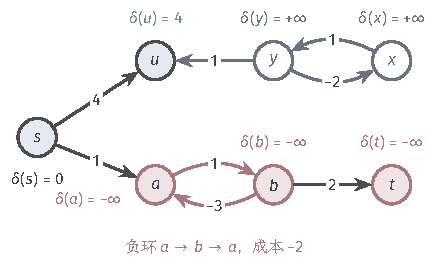
\includegraphics[width=73.801mm]{figures/01-basic-mathematics/04-graphs/tikz/c3-distance-outcomes/figure.pdf}
  \caption{单源最短路的三类结果同处一图（源点为$s$，弧旁数字为长度）。$a\to b\to a$的成本为$1-3=-2$，是从$s$可达的负环，环上的$a,b$及其后继$t$的距离为$-\infty$（红色）；旁支$u$不能从该负环到达，距离为有限值$4$（蓝色）；负环$x\to y\to x$从$s$不可达，$x,y$的距离为$+\infty$（灰色），弧$y\to u$也不会改变$u$的距离。}
  \label{fig:graph-opt-distance-outcomes}
\end{figure}

无向图中的负边需要特别注意。把无向边$\{u,v\}$换成两条同长的反向弧$u\to v$与$v\to u$以后，一条长为负的无向边自己就构成负环：沿它走过去再走回来，成本是两倍的负长度。因此，把含负边的无向图换成有向图后，本章的负环检测算法会将受影响的距离报告为$-\infty$，不能据此求出“只允许简单路径”时的最小值。下文只在无向边长度非负时用这类转换求有限最短路。

\subsection{距离标签与松弛}
\label{sec:graph-opt-sp-relaxation}
\label{sec:graph-opt-relaxation}

最短路算法都不直接枚举行走，而是为每个顶点保存一个当前已知的最好成本，在发现更好的路线时更新它。以固定源点$s$为例，设想已经知道一条从$s$到$u$、成本为$d(u)$的路线，又有弧$u\to v$，那么把这条弧接在路线末尾，就得到一条到$v$、成本为$d(u)+\ell_{u,v}$的路线。如果它比$v$目前记录的成本更低，就应该改用它。

\paragraph{松弛操作}
为每个顶点$v$保存一个\term{距离标签}（distance label）$d(v)\in\mathbb R\cup\{+\infty\}$和一个前驱$p(v)$（在全源最短路中则对每个源点$u$维护一行距离标签$d(u,v)$与前驱$\pi(u,v)$）。单源初始化时令$d(s)=0$，其余顶点$d(v)=+\infty$，前驱为空。对一条弧$u\to v$执行\term{松弛}（relaxation），是指比较当前标签$d(v)$与候选值$d(u)+\ell_{u,v}$：若$d(u)<+\infty$且
\begin{equation}
  d(u)+\ell_{u,v}<d(v),
  \label{eq:graph-opt-relaxation}
\end{equation}
就令$d(v)\leftarrow d(u)+\ell_{u,v}$、$p(v)\leftarrow u$；否则什么也不做。只有严格改善时才更新，因而标签只会下降，不会上升。

图~\ref{fig:graph-opt-relaxation}画出一次松弛的两种结果：候选值$5$小于原标签$8$时，标签与前驱一起改写；原标签已是$4$时，两者都不变。距离数组和前驱数组必须同步修改：如果只改距离而不改前驱，回溯得到的路线成本就不再等于标签。

\begin{figure}[!htb]
  \centering
  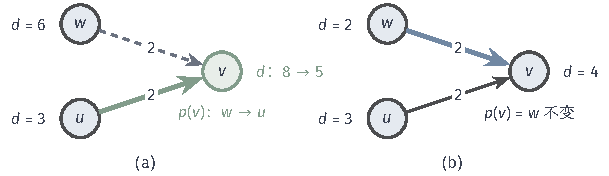
\includegraphics[width=102.993mm]{figures/01-basic-mathematics/04-graphs/tikz/c3-relaxation/figure.pdf}
  \caption{对弧$u\to v$松弛（顶点旁为当前标签，弧旁为长度）。(a) 候选值$d(u)+\ell_{u,v}=3+2=5$小于原标签$8$，标签改为$5$，前驱由$w$改为$u$（绿色表示被改善的标签与新的前驱弧，虚线为被替换的旧前驱弧）。(b) 原标签为$4$，候选值$5$不能改善，标签与前驱都不变。}
  \label{fig:graph-opt-relaxation}
\end{figure}

\paragraph{上界不变量与三角不等式最优性条件}
松弛只从有限标签出发延长路线，由此得到所有最短路算法共用的一个\emph{上界不变量}：每个有限标签$d(v)$都等于某条从$s$到$v$的行走的成本。初始时只有$d(s)=0$有限，对应零步行走。若松弛把$d(v)$改为$d(u)+\ell_{u,v}$，则把$u$的那条行走接上弧$u\to v$，就得到成本恰为新标签的行走。由此立即得到$d(v)\geq\delta(v)$：标签永远是真实距离的上界。后面每种算法要做的，都是说明在适当的条件下，这个上界最终会降到$\delta(v)$。

反过来，当没有一条弧还能通过松弛继续改善标签时，即对每条起点标签有限的弧$u\to v$都满足\emph{逐弧三角不等式}
\begin{equation}
  d(v)\leq d(u)+\ell_{u,v},
  \label{eq:graph-opt-shortest-path-certificate}
\end{equation}
且$d(s)=0$，则任取一条从$s$到$v$的行走$W=(s=w_0,w_1,\ldots,w_k=v)$，沿$W$把式~\eqref{eq:graph-opt-shortest-path-certificate}逐条相加，中间顶点的标签一正一负恰好裂项相消，得到
\[
  d(v)\leq d(s)+\ell(W)=\ell(W).
\]
对所有行走$W\in\mathcal W_{s,v}$取下确界即得下界$d(v)\leq\delta(v)$。结合上界不变量$d(v)\geq\delta(v)$，立即确认$d(v)=\delta(v)$。因此，“前驱路线见证上界”与“逐弧三角不等式式~\eqref{eq:graph-opt-shortest-path-certificate}提供下界”合在一起，就构成了不依赖具体算法过程的\emph{最短路最优性证书}。

需要注意，为什么算法不能脱离“从源为零、其余为无穷出发逐弧松弛”的过程，而直接去求解局部不动点方程
\[
  \delta(v)=\min_{u\to v}\{\delta(u)+\ell_{u,v}\}\quad(v\neq s),\qquad \delta(s)=0\text{？}
\]
原因在于满足这组局部等式的数组不一定有真实路线支撑。设$s\to a$长$5$，$a\to b$与$b\to a$长都为$0$，则对任意$c\leq5$，取$D(s)=0$、$D(a)=D(b)=c$都满足
\[
  D(a)=\min\{D(s)+5,\ D(b)+0\}=c,\qquad D(b)=D(a)+0=c,
\]
而真实距离是$\delta(a)=\delta(b)=5$。这里的零成本环让$a,b$互相“支撑”着一个过低的值，却没有任何从$s$出发的实际路线达到它。初值“源为零、其余为无穷”加松弛更新，恰好保证了每个有限标签都有实际路线见证。

各算法都同时保存标签与前驱。前驱$p(v)$记录最近一次改善该标签时所用的最后一条弧，用于事后恢复最短路树（shortest-path tree），但只在标签不再变化以后才能放心回溯：在一般有环图中，计算中途的前驱指针可能尚未形成从$s$出发的树；若存在可达负环，前驱指针甚至可能首尾相接成环。

% 第3章第2节：单源最短路（有向无环图递推；Bellman--Ford算法；Dijkstra算法；方法比较与结果检验）。

\section{单源最短路}
\label{sec:single-source-shortest-paths}

固定一个源点$s\in V$，单源最短路问题要求求出从$s$到每个顶点$v\in V$的最短距离$\delta(v)$与前驱$p(v)$。本节的三种算法都沿用第~\ref{sec:shortest-path-foundations}节的距离标签与松弛机制，差别只在于按什么次序对弧执行松弛、何时可以断定一个顶点的标签已经稳定不再改变：第~\ref{sec:graph-opt-dag-sp}小节在有向无环图上按拓扑序一遍扫描完成；第~\ref{sec:graph-opt-bellman-ford}小节在允许有环和负权弧的一般有向图上反复扫描全部弧并识别负环；第~\ref{sec:graph-opt-dijkstra}小节利用弧长非负的条件，借优先队列每次永久确定当前最小标签；第~\ref{sec:graph-opt-sssp-comparison}小节汇总对比三种单源算法与结果核验方法。

\subsection{有向无环图上的最短路}
\label{sec:graph-opt-dag-sp}
\label{sec:graph-opt-dag-shortest-path}

\subsubsection{问题与思路}

输入限定为有向无环图，弧长仍可为任意实数。在一般的图中，一个顶点的标签可能在它的出弧已被松弛之后才下降，这时它的后继也必须随之更新。有向无环图没有这个问题：第~\ref{sec:graph-topological-order}节说明，有限有向无环图存在拓扑序，使每条弧的起点排在终点之前。按拓扑序处理顶点，轮到$v$时，所有指向$v$的弧都已被松弛，$v$的标签此后不会再变，于是可以放心地用它去松弛$v$的出弧。

\subsubsection{算法实现}

拓扑序在松弛开始前一次求出，它只规定处理次序，运行中不再改变，因此不计入算法状态。算法维护三项状态：
\begin{itemize}
  \item 距离标签$d(v)$：初值$d(s)=0$，其余为$+\infty$；
  \item 前驱$p(v)$：初值为空；
  \item 位置$i$：下一个待处理的顶点在拓扑序中的序号，初值为$1$。
\end{itemize}
每一步处理拓扑序中的第$i$个顶点$v_i$：若$d(v_i)<+\infty$，对它的每条出弧执行松弛，否则它给不出有限候选，直接跳过；然后令$i\gets i+1$。处理完$v_n$后停止，再沿前驱恢复路线。

\begin{algorithm}[有向无环图上的最短路]
\label{alg:graph-opt-dag-shortest-path}
输入：有限有向无环图、弧长$\ell_{u,v}\in\mathbb R$、源点$s$。输出：全部距离$\delta(v)$与前驱$p(v)$。
\begin{enumerate}
  \item 求一个拓扑序$v_1,\ldots,v_n$；令$d(s)=0$，其余$d(v)=+\infty$，前驱为空。
  \item 按$i=1,\ldots,n$的顺序处理$v_i$：若$d(v_i)<+\infty$，对其每条出弧$v_i\to w$执行松弛。
  \item 对标签有限的顶点，沿前驱从终点退回$s$再反转，得到一条最短路；标签为$+\infty$的顶点报告不可达。
\end{enumerate}
\end{algorithm}

\paragraph{执行过程}
下面用一张四点图逐步演示，它的五条弧长为：
\[
  \ell_{s,a}=2,\quad\ell_{s,b}=5,\quad\ell_{a,b}=-1,\quad\ell_{a,t}=5,\quad\ell_{b,t}=2.
\]
这张图没有有向环，拓扑序可取$(s,a,b,t)$。初始标签为
\[
  (d(s),d(a),d(b),d(t))=(0,+\infty,+\infty,+\infty),
\]
前驱全为空。按拓扑序逐个处理顶点，松弛它的出弧：
\begin{itemize}
  \item 处理$s$：$a$由$+\infty$改为$0+2=2$，$b$由$+\infty$改为$0+5=5$，前驱都记为$s$，标签变为$(0,2,5,+\infty)$。
  \item 处理$a$：候选$2+(-1)=1<5$，$b$改为$1$、前驱改为$a$；$t$由$+\infty$改为$2+5=7$、前驱记为$a$。标签变为$(0,2,1,7)$。
  \item 处理$b$：候选$1+2=3<7$，$t$改为$3$、前驱改为$b$，标签变为$(0,2,1,3)$。
  \item 处理$t$：没有出弧，标签不变。
\end{itemize}
扫描结束时前驱为$p(a)=s$、$p(b)=a$、$p(t)=b$。从$t$回溯得到最短路$s\to a\to b\to t$，成本为
\[
  \ell_{s,a}+\ell_{a,b}+\ell_{b,t}=2-1+2=3.
\]
图~\ref{fig:graph-opt-dag-labels}记录了各标签的变化次序。

\begin{figure}[!htb]
  \centering
  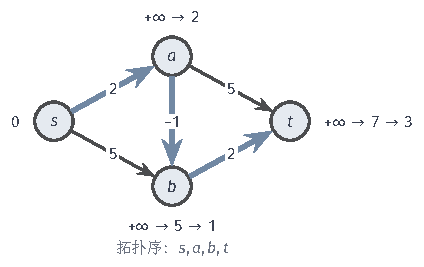
\includegraphics[width=71.635mm]{figures/01-basic-mathematics/04-graphs/tikz/c3-dag-labels/figure.pdf}
  \caption{按拓扑序$(s,a,b,t)$在有向无环图上松弛。顶点旁列出标签的变化次序，例如$b$先由处理$s$得到$5$，再由处理$a$改为$1$；蓝色粗弧是最终前驱弧，组成最短路$s\to a\to b\to t$（成本$3$）。负长度弧$a\to b$并不妨碍计算，因为正确性只依赖无环次序。}
  \label{fig:graph-opt-dag-labels}
\end{figure}

\subsubsection{算法分析}

\paragraph{正确性}
一遍扫描之所以够用，是因为处理到某个顶点时，所有可能到达它的路线都已考虑过。

\begin{theorem}[有向无环图上最短路的正确性]
\label{thm:graph-opt-dag-shortest-path}
设$\mathcal G$是有限有向无环图，弧长为任意实数。算法~\ref{alg:graph-opt-dag-shortest-path}结束时，对每个顶点$v$都有$d(v)=\delta(v)$；其中$\delta(v)=+\infty$当且仅当$v$从$s$不可达，其余$\delta(v)$均为有限值。
\end{theorem}

\begin{proof}
有向无环图中的行走不会重复顶点，因此每条行走都是简单路径，只有有限条，$\delta(v)$只可能是$+\infty$或有限值。松弛只改变弧终点的标签，而指向$v$的弧都从拓扑序中排在$v$之前的顶点出发，所以轮到$v$时它的标签已经不再改变。下面对拓扑序归纳，证明轮到$v$时$d(v)=\delta(v)$。

排在$s$之前的顶点从$s$不可达，它们的标签保持$+\infty$，与距离一致。对$v=s$，不存在回到$s$的非零步行走，故$\delta(s)=0=d(s)$。

设$v$排在$s$之后，并且此前的顶点都已满足结论。若$v$不可达，则它的标签不可能变为有限值，因为有限标签总对应一条实际行走。若$v$可达，任取一条$s$到$v$的路径，设其最后一条弧为$u\to v$，则$u$排在$v$之前，路径前缀的成本不小于$\delta(u)$，归纳假设给出$\delta(u)=d(u)$。处理$u$时弧$u\to v$已被松弛，因而
\[
  d(v)\leq d(u)+\ell_{u,v}=\delta(u)+\ell_{u,v}\leq\text{该路径的成本}.
\]
路径是任取的，所以$d(v)\leq\delta(v)$。结合标签不变量$d(v)\geq\delta(v)$，得$d(v)=\delta(v)$。
\end{proof}

证明中只用到“前驱先于后继处理”，没有用到边长的符号，所以负长度弧不会造成任何问题；反过来，图中只要有一个有向环就没有拓扑序，算法无法开始，此时要改用后面两种算法。

\paragraph{复杂度}
求拓扑序需要$O(n+a)$时间，之后每个顶点处理一次、每条弧松弛一次，总时间为$O(n+a)$，标签、前驱与拓扑序共占$O(n)$额外空间。

\subsubsection{编辑距离}

许多递推问题的状态之间天然形成有向无环图：每个状态的最优值，由能一步转来的前面状态加上这一步的代价取最小得到。这正是按拓扑序松弛的最短路问题，编辑距离是一个典型例子。

比较两段序列时，常问把序列$\bm a=(a_1,\ldots,a_p)$改写成$\bm b=(b_1,\ldots,b_q)$最少需要多少次单元素操作，允许的操作是插入一个元素、删除一个元素和把一个元素替换为另一个。

以$(i,j)$表示“已把$\bm a$的前$i$个元素改写成$\bm b$的前$j$个元素”这一状态，最后一步只有三种可能：删去$a_i$，从$(i-1,j)$而来，成本为$1$；插入$b_j$，从$(i,j-1)$而来，成本为$1$；让$a_i$对应$b_j$，从$(i-1,j-1)$而来，相同时成本为$0$，不同时为一次替换，成本为$1$。

于是最少操作数$E(i,j)$满足
\begin{equation}
  E(i,j)=\min\bigl\{E(i-1,j)+1,\ E(i,j-1)+1,\ E(i-1,j-1)+\mathbb I\{a_i\neq b_j\}\bigr\},
  \label{eq:graph-opt-edit-distance}
\end{equation}
边界为$E(i,0)=i$、$E(0,j)=j$，其中$\mathbb I\{\cdot\}$在条件成立时取$1$、否则取$0$。

每条状态弧都使$i+j$增加，所以状态图没有有向环，$E(p,q)$就是从$(0,0)$到$(p,q)$的最短路距离，称为两段序列的\term{编辑距离}（edit distance）。

按$i+j$递增或逐行的顺序计算，正是在按拓扑序松弛。例如$\bm a=(A,B)$、$\bm b=(A,C,B)$时，逐行计算得到表~\ref{tab:graph-opt-edit-distance}，沿“匹配$A$、插入$C$、匹配$B$”得到距离$E(2,3)=1$。

全表连同前驱需要$O((p+1)(q+1))$时间与空间（$p,q\geq1$时为$O(pq)$）；只要距离值时保留相邻两行即可。若为插入、删除和替换分别指定固定的非负成本，只需改变相应状态弧的长度，状态图仍然无环，计算次序不变。

\begin{table}[!htb]
  \centering
  \begin{tabular}{@{}ccccc@{}}
    \toprule
    & $j=0$ & $j=1$（$A$） & $j=2$（$C$） & $j=3$（$B$） \\
    \midrule
    $i=0$ & $0$ & $1$ & $2$ & $3$ \\
    $i=1$（$A$） & $1$ & $0$ & $1$ & $2$ \\
    $i=2$（$B$） & $2$ & $1$ & $1$ & $1$ \\
    \bottomrule
  \end{tabular}
  \caption{$\bm a=(A,B)$改写为$\bm b=(A,C,B)$的编辑距离表。第$i$行第$j$列为$E(i,j)$，按式~\eqref{eq:graph-opt-edit-distance}逐行计算；右下角$E(2,3)=1$。}
  \label{tab:graph-opt-edit-distance}
\end{table}

\subsection{Bellman--Ford算法}
\label{sec:graph-opt-bellman-ford}

\subsubsection{问题与思路}

一般的有向图可能有环，没有拓扑序可用，一遍扫描不够。最直接的补救是反复扫描全部弧，让后来的改善继续向后传递，直到标签不再变化。为了说清每一轮扫描得到了什么，考虑各轮彼此分开的同步版本：第$k$轮只读取第$k-1$轮结束时的标签。这样，第$k$轮的标签恰好考虑了至多$k$条弧的路线；不受负环影响的顶点由至多$n-1$条弧的简单路径达到，所以$n-1$轮就够了。完成这些轮次后再扫描一次，仍能改善的弧就暴露了负环的影响。

\subsubsection{算法实现}

同步版本的第$k$轮对每个顶点比较“沿用旧值”与“在上一轮的某条路线后再接一条弧”：
\begin{equation}
  d^{(k)}(v)=\min\Bigl\{d^{(k-1)}(v),\ \min_{u\to v}\bigl(d^{(k-1)}(u)+\ell_{u,v}\bigr)\Bigr\},\qquad k=1,2,\ldots,
  \label{eq:graph-opt-bellman-ford}
\end{equation}
没有入弧时内层最小值取$+\infty$。算法维护四项状态：
\begin{itemize}
  \item 两份标签数组$d^{(k-1)}$与$d^{(k)}$：本轮只读前者、只写后者，初值$d^{(0)}(s)=0$，其余为$+\infty$；
  \item 前驱$p(v)$：最近一次改善$d(v)$时提供候选值的顶点，初值为空；
  \item 轮次$k$：已完成的轮数，初值为$0$；
  \item 改善标记：本轮有无标签改变。
\end{itemize}
每一轮依次做三件事：
\begin{itemize}
  \item 复制：令$k\gets k+1$，把$d^{(k-1)}$复制为$d^{(k)}$，改善标记置为否。
  \item 逐弧更新：对每条起点标签有限的弧$u\to v$，若$d^{(k-1)}(u)+\ell_{u,v}<d^{(k)}(v)$，就令$d^{(k)}(v)\gets d^{(k-1)}(u)+\ell_{u,v}$、$p(v)\gets u$，并记下有改善。扫描完全部弧，$d^{(k)}$恰为式~\eqref{eq:graph-opt-bellman-ford}的右端。
  \item 停止判断：若$k=n-1$或本轮无改善，停止递推；否则进入下一轮。
\end{itemize}
递推停止后，固定此时的标签$d$，分两步判别负环的影响：
\begin{itemize}
  \item 找种子：起点标签有限、仍满足$d(u)+\ell_{u,v}<d(v)$的弧$u\to v$，其终点称为种子。递推提前停止时没有种子。
  \item 标记：从全部种子出发沿出弧遍历，把到达的顶点标记为$-\infty$。
\end{itemize}
其余顶点中，标签为$+\infty$的报告不可达，标签有限的以标签为距离。

\begin{algorithm}[Bellman--Ford算法]
\label{alg:graph-opt-bellman-ford}
输入：有向图的出邻接表与弧长$\ell$，起点$s$。输出：每个顶点的距离或“不可达”“$-\infty$”，以及前驱。
\begin{enumerate}
  \item 置$d^{(0)}(s)=0$，其余$d^{(0)}(v)=+\infty$，前驱为空，$k=0$。若$n=1$，直接令$d=d^{(0)}$并转至第4步。
  \item 令$k\gets k+1$，把$d^{(k-1)}$复制为$d^{(k)}$。对每条$d^{(k-1)}(u)<+\infty$的弧$u\to v$，若$d^{(k-1)}(u)+\ell_{u,v}<d^{(k)}(v)$，置$d^{(k)}(v)=d^{(k-1)}(u)+\ell_{u,v}$、$p(v)=u$。
  \item 若本轮有标签改善且$k<n-1$，回到第2步；否则记$d=d^{(k)}$。
  \item 把满足$d(u)<+\infty$且$d(u)+\ell_{u,v}<d(v)$的弧$u\to v$的终点作为种子，从全部种子沿出弧遍历，到达的顶点标为$-\infty$；其余顶点按$d$报告距离或不可达。
\end{enumerate}
\end{algorithm}

\paragraph{执行过程}
上一小节的四点图没有环，看不出反复扫描的必要。图~\ref{fig:graph-opt-bellman-ford-rounds}换用一个有环的例子，它有五个顶点和六条弧，弧长为：
\[
  \begin{gathered}
    \ell_{s,t}=6,\quad\ell_{s,b}=2,\quad\ell_{b,c}=3,\\
    \ell_{c,a}=-4,\quad\ell_{a,t}=2,\quad\ell_{t,b}=1.
  \end{gathered}
\]
其中$b\to c\to a\to t\to b$构成一个环，成本为$3-4+2+1=2$，不是负环。按式~\eqref{eq:graph-opt-bellman-ford}逐轮计算，各轮标签见表~\ref{tab:graph-opt-bellman-ford-rounds}。

第$1$轮只能用一条弧：$t$由$s$得到$6$，$b$由$s$得到$2$，其余仍为$+\infty$。
\begin{BookInlineFigure}
  \centering
  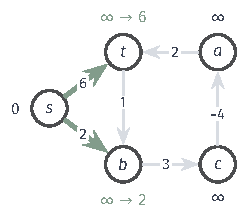
\includegraphics[width=40.771mm]{figures/03-graphs/02-combinatorial-optimization/tikz/reading-steps/bellman-ford-round-1.pdf}
  \caption{Bellman--Ford第$1$轮结束。本轮只能沿从$s$出发的单条弧产生有限候选。弧旁数字是弧长，顶点旁是标签；绿色弧与数字表示本轮改善，蓝色弧表示此前保留的前驱。}
  \label{fig:graph-opt-bellman-ford-rounds}
\end{BookInlineFigure}

第$2$轮：$c$经$b$得到$2+3=5$。$a\to t$与$c\to a$的起点在上一轮还是$+\infty$，不产生候选。
\begin{BookInlineFigure}
  \centering
  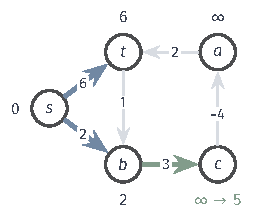
\includegraphics[width=42.774mm]{figures/03-graphs/02-combinatorial-optimization/tikz/reading-steps/bellman-ford-round-2.pdf}
  \caption{第$2$轮：改善从$b$传到$c$，得到$d(c)=5$。本轮仍读取上一轮的标签，因此不能立刻沿$c\to a$继续传递。}
  \label{fig:graph-opt-bellman-ford-rounds-2}
\end{BookInlineFigure}

第$3$轮：$a$经$c$得到$5-4=1$，对应三弧路线$s\to b\to c\to a$。
\begin{BookInlineFigure}
  \centering
  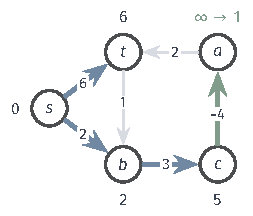
\includegraphics[width=42.774mm]{figures/03-graphs/02-combinatorial-optimization/tikz/reading-steps/bellman-ford-round-3.pdf}
  \caption{第$3$轮：沿$c\to a$得到$d(a)=1$。此前$t$的标签仍为直达路线的成本$6$。}
  \label{fig:graph-opt-bellman-ford-rounds-3}
\end{BookInlineFigure}

第$4$轮：$t$经$a$降到$1+2=3$，前驱由$s$改为$a$，对应四弧路线$s\to b\to c\to a\to t$，比直达的$s\to t$便宜。
\begin{BookInlineFigure}
  \centering
  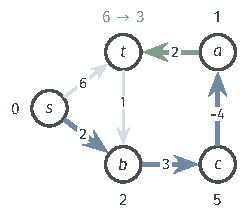
\includegraphics[width=40.771mm]{figures/03-graphs/02-combinatorial-optimization/tikz/reading-steps/bellman-ford-round-4.pdf}
  \caption{第$4$轮：沿$a\to t$把$d(t)$由$6$降为$3$，并改写$t$的前驱。蓝绿弧组成最终最短路径树。}
  \label{fig:graph-opt-bellman-ford-rounds-4}
\end{BookInlineFigure}

此时$k=4=n-1$，递推停止。再检查全部弧，没有一条还能改善，因而没有种子，最终距离为$(s,a,b,c,t)=(0,1,2,5,3)$。

这个例子恰好用满了$n-1$轮，因为$t$的最短路含$4$条弧；每一行都是“至多$k$条弧”的最优值，例如$d^{(3)}(t)=6$只计入了单弧路线$s\to t$。改善沿环$b\to c\to a\to t$传递了一圈，但回到$b$时，候选$3+1=4$不小于$2$，传递就此停止：环的成本非负，绕圈不会更便宜。

\begin{table}[!htb]
  \centering
  \begin{tabular}{cccccc}
    \toprule
    轮次$k$ & $d^{(k)}(s)$ & $d^{(k)}(a)$ & $d^{(k)}(b)$ & $d^{(k)}(c)$ & $d^{(k)}(t)$ \\
    \midrule
    $0$ & $0$ & $+\infty$ & $+\infty$ & $+\infty$ & $+\infty$ \\
    $1$ & $0$ & $+\infty$ & $2$（$s$） & $+\infty$ & $6$（$s$） \\
    $2$ & $0$ & $+\infty$ & $2$ & $5$（$b$） & $6$ \\
    $3$ & $0$ & $1$（$c$） & $2$ & $5$ & $6$ \\
    $4$ & $0$ & $1$ & $2$ & $5$ & $3$（$a$） \\
    \bottomrule
  \end{tabular}
  \caption{同步Bellman--Ford在图~\ref{fig:graph-opt-bellman-ford-rounds}的含环图上的逐轮标签。第$k$行是至多$k$条弧的最小成本，括号内为该轮改变标签时的前驱。}
  \label{tab:graph-opt-bellman-ford-rounds}
\end{table}

负环存在时，标签不会停下来。回到图~\ref{fig:graph-opt-distance-outcomes}。该图有$7$个顶点，同步计算$6$轮，各轮标签见表~\ref{tab:graph-opt-bellman-ford-negative}。$u$在第$1$轮得到$4$后不再变化，$x,y$始终为$+\infty$；而$a,b,t$的标签每隔一两轮就再降一次，第$6$轮停在$-3,-2,2$。这几个数只反映绕圈到第$6$轮时标签降到了哪里，并不是任何意义下的距离。

此时检查全部弧，$b\to a$与$b\to t$的候选分别为
\[
  -2-3=-5<-3,\qquad -2+2=0<2,
\]
两条弧仍可改善，种子是$a$与$t$；其余弧都不能改善。从种子沿出弧遍历，标记出$\{a,b,t\}$。算法报告$u$的距离为$4$，$a,b,t$为$-\infty$，$x,y$不可达，与前面的分析一致。

\begin{table}[!htb]
  \centering
  \begin{tabular}{cccccc}
    \toprule
    轮次$k$ & $d^{(k)}(s)$ & $d^{(k)}(u)$ & $d^{(k)}(a)$ & $d^{(k)}(b)$ & $d^{(k)}(t)$ \\
    \midrule
    $0$ & $0$ & $+\infty$ & $+\infty$ & $+\infty$ & $+\infty$ \\
    $1$ & $0$ & $4$ & $1$ & $+\infty$ & $+\infty$ \\
    $2$ & $0$ & $4$ & $1$ & $2$ & $+\infty$ \\
    $3$ & $0$ & $4$ & $-1$ & $2$ & $4$ \\
    $4$ & $0$ & $4$ & $-1$ & $0$ & $4$ \\
    $5$ & $0$ & $4$ & $-3$ & $0$ & $2$ \\
    $6$ & $0$ & $4$ & $-3$ & $-2$ & $2$ \\
    \bottomrule
  \end{tabular}
  \caption{同步Bellman--Ford在图~\ref{fig:graph-opt-distance-outcomes}上的逐轮标签（$x,y$各轮均为$+\infty$，未列出）。$u$在第$1$轮后稳定；可达负环$a\to b\to a$使$a,b,t$的标签持续下降。}
  \label{tab:graph-opt-bellman-ford-negative}
\end{table}

\paragraph{就地更新}
常见的实现不复制数组，而是在同一个数组上逐弧松弛，一轮中刚改善的标签可以立即被同一轮后面的弧使用，称为就地更新。

扫描次序会影响所需轮数。按$s\to t$、$s\to b$、$b\to c$、$c\to a$、$a\to t$、$t\to b$的顺序扫描上例，第一轮就依次得到$t=6$、$b=2$、$c=5$、$a=1$，并把$t$降到$3$，即全部最终标签，第二轮无改善即可停止。若按相反的顺序扫描，每轮只能把改善推进一步，仍要四轮。

它的停止规则与负环检测方式和同步版本相同，只是“第$k$轮”的含义变了。

\subsubsection{算法分析}

\paragraph{正确性}
分析从同步版本出发，因为它的标签有一个清楚的含义。

\begin{lemma}[同步标签的含义]
\label{lem:graph-opt-bellman-ford-k-arcs}
对每个$k\geq0$与每个顶点$v$，$d^{(k)}(v)$等于从$s$到$v$、至多含$k$条弧的全部行走的最小成本；没有这样的行走时为$+\infty$。
\end{lemma}

\begin{proof}
对$k$归纳。$k=0$时，至多零条弧的行走只有$s$处的零步行走，与$d^{(0)}$一致。设结论对$k-1$成立。一条至多含$k$条弧、到达$v$的行走，要么至多含$k-1$条弧，其成本不小于$d^{(k-1)}(v)$；要么恰含$k$条弧，去掉最后一条弧$u\to v$后剩下至多$k-1$条弧、到达$u$的前缀，原行走的成本不小于$d^{(k-1)}(u)+\ell_{u,v}$。所以全部候选的最小值不小于式~\eqref{eq:graph-opt-bellman-ford}的右端。反过来，右端每个有限候选都由归纳假设对应一条至多$k$条弧的行走；存在有限候选时最小值能够达到，否则两边都为$+\infty$。故两者相等。
\end{proof}

由此先得到轮数上界。对可达且不受可达负环影响的顶点$v$，第~\ref{sec:graph-opt-sp-problem}小节说明$\delta(v)$由一条简单路径达到，而简单路径至多经过$n$个顶点、含$n-1$条弧。由引理~\ref{lem:graph-opt-bellman-ford-k-arcs}，第$n-1$轮已经计入这条路径，所以$d^{(n-1)}(v)=\delta(v)$。若某一整轮没有任何标签改变，则此后各轮的输入都相同，标签不会再变，提前停止不影响结果；此时由下面的定理，图中不存在可达负环。

就地更新得到的标签仍是真实行走的成本，又对每轮都不高于同步版本的标签（对轮数归纳即可），所以$n-1$轮的上界照样成立。但“第$k$轮标签恰为至多$k$条弧的最优值”这一解释只属于同步版本，不能原样套在就地更新上：同一轮内的改善可能已经串起了多条弧。

\paragraph{负环的判别}
$n-1$轮之后的种子与遍历恰好找出了全部距离为$-\infty$的顶点。

\begin{theorem}[Bellman--Ford算法对三类结果的判定]
\label{thm:graph-opt-bellman-ford-negative-cycles}
在同步递推的$n-1$轮之后按上述方法标记，被标记的顶点恰好是$\delta(v)=-\infty$的顶点；其余顶点中，$d^{(n-1)}(v)=+\infty$的不可达，$d^{(n-1)}(v)$有限的满足$d^{(n-1)}(v)=\delta(v)$。
\end{theorem}

\begin{proof}
先证每个种子$v$都满足$\delta(v)=-\infty$。由引理~\ref{lem:graph-opt-bellman-ford-k-arcs}，$v$可改善说明$d^{(n)}(v)<d^{(n-1)}(v)$，即存在一条恰含$n$条弧的行走，比所有至多$n-1$条弧的行走都便宜。

含$n$条弧的行走经过$n+1$个顶点位置，必有顶点重复，从中可以切出一段闭行走$C$。若$C$的成本非负，删去它会得到弧更少、成本不更高的行走，与上述“更便宜”矛盾；故$C$的成本为负，由第~\ref{sec:graph-opt-sp-problem}小节的分解，$C$中含有一个负环。这个负环位于一条从$s$出发、到达$v$的行走上，所以$\delta(v)=-\infty$。从种子沿出弧能到达的顶点也能从同一个负环到达，因而被标记的顶点距离都是$-\infty$。

再证每个$\delta(v)=-\infty$的顶点都会被标记。此时存在从$s$可达的负环$C=(c_0,c_1,\ldots,c_k=c_0)$能到达$v$。$C$上的顶点从$s$可达，可达顶点至多经$n-1$条弧到达，所以它们的标签有限。若$C$上没有一条弧可改善，则对每条环弧都有
\[
  d(c_{r})\leq d(c_{r-1})+\ell_{c_{r-1},c_r},\qquad r=1,\ldots,k.
\]
沿环把这$k$个不等式相加，两侧的标签之和恰好相消，得到$0\leq\ell(C)<0$，矛盾。因此$C$上至少有一个种子，而$v$能从$C$到达，必然被遍历标记。

最后，未被标记且可达的顶点不受任何可达负环影响，前面已说明$d^{(n-1)}(v)=\delta(v)$；不可达顶点的标签始终为$+\infty$。
\end{proof}

\paragraph{复杂度}
每轮逐弧扫描一次，用时$O(a)$，至多$n-1$轮，再加上一轮检测与一次遍历，计入初始化和末尾遍历，就地更新版本的总时间为$O(n+na)$。同步版本每轮还要复制标签数组，总时间上界为$O(n(n+a))$；若先限制在源点可达的子图上计算，则可避免每轮复制大量不可达顶点。只保存当前和上一轮的标签时，工作状态为$O(n)$。

\paragraph{路线恢复}
若要按引理~\ref{lem:graph-opt-bellman-ford-k-arcs}的含义回溯“至多$k$条弧”的最优路线，就需要保存每一轮的前驱$p^{(k)}(v)$，记录可达$O(n^2)$条。只保存一份前驱数组时，也可以回溯有限距离的顶点，但要说明这份前驱与递推相容。

设$v$未被标记且标签有限，若$p(v)=u$，则$u\to v$是一条弧，$u$也不会被标记，否则$v$能从负环到达。设置$p(w)=u$时，$d(w)$等于$u$此前某一时刻的标签加上$\ell_{u,w}$；标签只降不升，$d(w)$再下降时前驱又会改写，所以任一时刻每条前驱弧都满足
\[
  d(p(w))+\ell_{p(w),w}\leq d(w).
\]

前驱指针在未标记顶点之间不会成环：若成环，考察环上最后被设置的那个指针，在它被设置之前，环上其余前驱弧都满足上述不等式，而这条弧满足严格不等式，沿环相加，标签相消，得到环的成本为负；这个负环从$s$可达，又能沿前驱弧到达$v$，与$v$未被标记矛盾。于是从$v$沿前驱必能回到$s$。把沿途的不等式相加，所得路线的成本不超过$d(v)=\delta(v)$，因而恰好是一条最短路。

对标为$-\infty$的顶点，算法报告$-\infty$及传播标记，而不输出最短路。若还要输出可独立核验的负环证据，需额外保存更新历史或另行提取负环，并补出从$s$到该环、再从该环到目标顶点的行走；单个种子本身不构成完整证据。

\subsection{Dijkstra算法}
\label{sec:graph-opt-dijkstra}

\subsubsection{问题与思路}

Bellman--Ford算法要反复扫描全部弧，因为一个标签随时可能再被改小。若边长都非负，情况就不同了：在尚未确定的顶点中，标签最小的那个已经不可能再被改小，因为任何绕道而来的路线都要先经过某个标签不更小的顶点，后半程又不会让成本下降。Dijkstra算法利用这一点，每次把这样一个顶点永久确定下来，只松弛它的出弧，于是每条弧只需松弛一次。

Dijkstra算法所需的条件是从源点可达部分的弧长都非负。全图非负是便于检查的充分条件；从$s$到达不了的区域即使有负边，也不影响本次查询。在这一条件下，从$s$可达的部分不含负环，所有距离都是$+\infty$或有限值，输出只有两类。

\subsubsection{算法实现}

\paragraph{优先队列的数据结构}
取出标签最小的未确定顶点、在标签下降时调整它的位置，都由以标签为键的优先队列完成，常见的实现有两种。一种是支持“降键”的索引堆，每个顶点在堆中只有一个条目，标签改善时原地下调它的键。另一种不降键，标签改善时直接插入一个新条目$(d(v),v)$，旧条目留在堆中；出队时若发现该顶点已经确定，说明这是过期条目，直接丢弃。两种实现的输出相同，区别只在队列规模与操作次数。

\paragraph{Dijkstra算法的实现}
算法维护四项状态：
\begin{itemize}
  \item 距离标签$d(v)$：初值$d(s)=0$，其余为$+\infty$；
  \item 前驱$p(v)$：初值为空；
  \item 已确定集合$R$：标签已永久确定的顶点，初值为空集；
  \item 优先队列：以标签为键存放标签有限的未确定顶点，初值只含$s$。
\end{itemize}
每一步做两件事：
\begin{itemize}
  \item 确定：取出队列中标签最小的顶点$u$，把它加入$R$；
  \item 松弛：对$u$通往$R$外的每条出弧执行松弛，标签改善时相应调整队列。
\end{itemize}
队列中不再有标签有限的未确定顶点时停止。

\begin{algorithm}[Dijkstra算法]
\label{alg:graph-opt-dijkstra}
输入：有限有向图、源点$s$，从$s$可达部分的弧长非负。输出：全部距离$\delta(v)$与前驱$p(v)$。
\begin{enumerate}
  \item 令$d(s)=0$，其余$d(v)=+\infty$，$R=\varnothing$。
  \item 当存在标签有限的未确定顶点时，取出其中标签最小的$u$，把$u$加入$R$。
  \item 对$u$的每条出弧$u\to v$，若$v\notin R$，执行松弛；标签改善时更新优先队列中$v$的键。
  \item 结束时，$R$中顶点的标签即为距离，其余顶点不可达。
\end{enumerate}
\end{algorithm}

\paragraph{执行过程}
把四点图中$a\to b$的长度由$-1$改为$1$，全部弧长非负，Dijkstra算法适用。表~\ref{tab:graph-opt-dijkstra-trace}列出每次出队后的状态。

第$1$步取出$s$，松弛得$d(a)=2$、$d(b)=5$，前驱都是$s$。
\begin{BookInlineFigure}
  \centering
  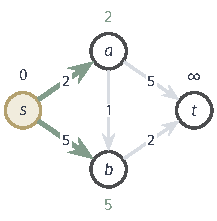
\includegraphics[width=36.784mm]{figures/03-graphs/02-combinatorial-optimization/tikz/reading-steps/dijkstra-step-1.pdf}
  \caption{Dijkstra第$1$步：取出$s$并松弛两条出弧。黄色是本次出队顶点，蓝底是已确定顶点；绿色标签和弧表示本次改善及新前驱。弧旁数字为长度，顶点旁为距离标签。}
  \label{fig:graph-opt-dijkstra-trace}
\end{BookInlineFigure}

第$2$步取出标签最小的$a$，候选$2+1=3<5$使$d(b)=3$、$p(b)=a$，候选$2+5=7$使$d(t)=7$、$p(t)=a$。
\begin{BookInlineFigure}
  \centering
  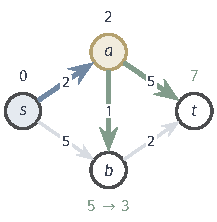
\includegraphics[width=36.784mm]{figures/03-graphs/02-combinatorial-optimization/tikz/reading-steps/dijkstra-step-2.pdf}
  \caption{第$2$步：确定$a$，经$a$把$b$的标签从$5$降为$3$，并首次到达$t$。已确定的$s,a$不再改写。}
  \label{fig:graph-opt-dijkstra-trace-2}
\end{BookInlineFigure}

第$3$步取出$b$，候选$3+2=5<7$使$d(t)=5$、$p(t)=b$。
\begin{BookInlineFigure}
  \centering
  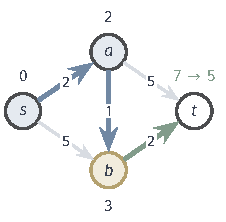
\includegraphics[width=38.347mm]{figures/03-graphs/02-combinatorial-optimization/tikz/reading-steps/dijkstra-step-3.pdf}
  \caption{第$3$步：确定$b$，经$b$把$t$的标签从$7$降为$5$。绿色弧$b\to t$替换此前的前驱弧$a\to t$。}
  \label{fig:graph-opt-dijkstra-trace-3}
\end{BookInlineFigure}

第$4$步取出$t$，它没有出弧，队列为空，停止。
\begin{BookInlineFigure}
  \centering
  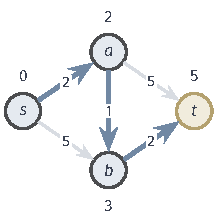
\includegraphics[width=36.784mm]{figures/03-graphs/02-combinatorial-optimization/tikz/reading-steps/dijkstra-step-4.pdf}
  \caption{第$4$步：确定$t$。最终前驱弧组成$s\to a\to b\to t$，各顶点标签均已等于最短距离。}
  \label{fig:graph-opt-dijkstra-trace-4}
\end{BookInlineFigure}

最终$\delta(a)=2$、$\delta(b)=3$、$\delta(t)=5$，从$t$沿前驱回溯得到$s\to a\to b\to t$。

图~\ref{fig:graph-opt-dijkstra-trace}至图~\ref{fig:graph-opt-dijkstra-trace-4}分别对应这四步：已确定集合$R$逐个向外扩张，每个顶点在出队时的标签都不再改变。

\begin{table}[!htb]
  \centering
  \begin{tabular}{@{}ccccccc@{}}
    \toprule
    步 & 出队 & $d(s)$ & $d(a)$ & $d(b)$ & $d(t)$ & $R$ \\
    \midrule
    初始 & — & $0$ & $+\infty$ & $+\infty$ & $+\infty$ & $\varnothing$ \\
    $1$ & $s$ & $0$ & $2$（$s$） & $5$（$s$） & $+\infty$ & $\{s\}$ \\
    $2$ & $a$ & $0$ & $2$ & $3$（$a$） & $7$（$a$） & $\{s,a\}$ \\
    $3$ & $b$ & $0$ & $2$ & $3$ & $5$（$b$） & $\{s,a,b\}$ \\
    $4$ & $t$ & $0$ & $2$ & $3$ & $5$ & $\{s,a,b,t\}$ \\
    \bottomrule
  \end{tabular}
  \caption{Dijkstra算法在非负四点图（$a\to b$长$1$，其余弧长同前）上的状态。每行是一次出队并松弛之后的标签与已确定集合，括号内为本步改变标签时的新前驱。}
  \label{tab:graph-opt-dijkstra-trace}
\end{table}

\subsubsection{算法分析}

\paragraph{正确性}
关键论断是：顶点被加入$R$的那一刻，它的标签已经等于真实距离，此后不再需要修正。证明的切入点是一条假设更短的路线上第一个尚未确定的顶点。

\begin{theorem}[Dijkstra算法的正确性]
\label{thm:graph-opt-dijkstra}
若从$s$可达部分的弧长都非负，则算法~\ref{alg:graph-opt-dijkstra}中每个顶点$u$被加入$R$时都有$d(u)=\delta(u)$；算法结束时未加入$R$的顶点从$s$不可达。
\end{theorem}

\begin{proof}
对加入$R$的次序归纳。第一个加入的是$s$，$d(s)=0=\delta(s)$，因为可达部分没有负环。设此前加入$R$的顶点都满足$d=\delta$，现在$u$被选出，且$d(u)<+\infty$。由标签不变量，$d(u)\geq\delta(u)$。假设$d(u)>\delta(u)$，取一条$s$到$u$、成本为$\delta(u)$的简单路径$P$。$P$从$s\in R$出发，到达$u\notin R$，所以沿$P$存在第一个不在$R$中的顶点$y$，记它在$P$上的前一个顶点为$x\in R$。

$x$加入$R$时弧$x\to y$已被松弛，此后标签只会下降。归纳假设给出$d(x)=\delta(x)$；而最短路的前缀仍是最短路，故$\delta(x)+\ell_{x,y}=\delta(y)$。于是
\[
  d(y)\leq d(x)+\ell_{x,y}=\delta(x)+\ell_{x,y}=\delta(y).
\]
$P$从$y$到$u$的后半段由可达部分的弧组成，长度非负，因而$\delta(y)\leq\delta(u)$。合起来得到
\[
  d(y)\leq\delta(y)\leq\delta(u)<d(u).
\]
但$y$也是未确定顶点，而算法选出的$u$在未确定顶点中标签最小，应有$d(u)\leq d(y)$，矛盾。所以$d(u)=\delta(u)$。

若算法停止时某个可达顶点$v$不在$R$中，取一条$s$到$v$的路径，同样找出第一个不在$R$中的顶点$y$及其前驱$x\in R$。松弛$x\to y$已使$d(y)$有限，算法便不会在此时停止，矛盾。
\end{proof}

\paragraph{适用范围}
证明中只有一步用到非负性：“后半段长度非负，所以$\delta(y)\leq\delta(u)$”。这一步失效时，算法确实会出错，即使图中没有负环。

下面的三弧图（图~\ref{fig:graph-opt-dijkstra-counterexample}）说明这一点，它的弧长为：
\[
  \ell_{s,a}=2,\quad\ell_{s,b}=5,\quad\ell_{b,a}=-4.
\]
处理$s$后，$a$的标签为$2$、$b$为$5$；算法选出标签较小的$a$并永久确定$d(a)=2$。随后处理$b$时，候选$5+(-4)=1$本可改善$a$，但$a$已在$R$中，不再更新。真实距离是$\delta(a)=1$，由路线$s\to b\to a$达到。

对照证明，这里的$y=b$、$u=a$，后半段$b\to a$为负，使$\delta(b)=5>\delta(a)=1$，“首个未确定顶点的标签不超过$\delta(u)$”不再成立。

\begin{figure}[!htb]
  \centering
  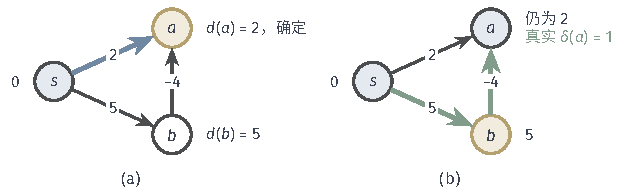
\includegraphics[width=105.583mm]{figures/01-basic-mathematics/04-graphs/tikz/c3-dijkstra-counterexample/figure.pdf}
  \caption{负边使Dijkstra算法过早确定标签。(a) 处理$s$后，$a$的标签$2$小于$b$的标签$5$，$a$被永久确定（黄色为当前出队顶点）。(b) 处理$b$时候选值$5-4=1$已无法改写$a$；真实最短路是$s\to b\to a$（绿色），成本$1$。图中没有负环，出错的原因是后半段弧$b\to a$为负。}
  \label{fig:graph-opt-dijkstra-counterexample}
\end{figure}

\paragraph{复杂度}
每个顶点至多出队一次，每条弧在其起点出队时松弛一次。用邻接表存储图、用支持降键的索引二叉堆存储未确定顶点时，取最小与降键各需$O(\log n)$时间，总时间为$O((n+a)\log n)$；标签、前驱、堆及其位置索引共占$O(n)$额外空间，图本身的存储另计。

不降键的实现每次改善插入一个条目，堆中至多有$a+1$个条目，操作时间为$O(\log a)=O(\log n)$，总时间仍为$O((n+a)\log n)$，但队列空间上界变为$O(a)$。稠密图上也可以不用堆，每次扫描数组找最小标签，总时间为$O(n^2+a)$。

\subsection{方法比较与结果检验}
\label{sec:graph-opt-sssp-comparison}
\label{sec:graph-opt-shortest-path-comparison}

三种算法解决同一个单源问题，但对输入的要求不同。比较它们时应先问：图有没有有向环？可达部分有没有负长度弧？是否需要检测负环？然后才比较运行时间。表~\ref{tab:graph-opt-shortest-path-methods}汇总了这些区别。

\begin{table}[!htb]
  \centering
  \begin{tabular}{llll}
    \toprule
    & 有向无环图递推 & Bellman--Ford & Dijkstra \\
    \midrule
    图结构 & 无有向环 & 不限 & 不限 \\
    弧长 & 任意实数 & 任意实数 & 可达部分非负 \\
    标签修正 & 处理后不变 & 反复修正 & 出队后不变 \\
    负环 & 不会出现 & 检测并标记 & 条件排除 \\
    时间 & $O(n+a)$ & $O(n+na)$ & $O((n+a)\log n)$ \\
    正确性依据 & 拓扑序归纳 & 至多$k$弧递推 & 首个未定顶点 \\
    \bottomrule
  \end{tabular}
  \caption{三种单源最短路算法的比较（$n$为顶点数，$a$为弧数，邻接表存储；Bellman--Ford采用就地更新版本）。}
  \label{tab:graph-opt-shortest-path-methods}
\end{table}

“允许负边”与“存在负环”是两件不同的事。有向无环图递推与Bellman--Ford算法都允许负边；前者因为无环而不会遇到负环，后者则能在负环存在时正确报告受影响的顶点。Dijkstra算法连负边都不允许，哪怕负边并不构成负环，图~\ref{fig:graph-opt-dijkstra-counterexample}就是这样的例子。一种算法在某组数据上跑得更快、甚至答案碰巧正确，都不能替代对其条件的检查。

拿到一份声称的单源最短路结果后，可以按第~\ref{sec:graph-opt-sp-relaxation}小节的最优性条件不重跑算法而直接核对。对标签有限的顶点，先沿前驱恢复路线，检查起点为$s$、终点为$v$、每一步都是原图中的弧，并重算弧长之和是否等于$d(v)$，证明$d(v)\geq\delta(v)$；再检查$d(s)=0$及每条起点标签有限的弧$u\to v$满足逐弧三角不等式~\eqref{eq:graph-opt-shortest-path-certificate}（$d(v)\leq d(u)+\ell_{u,v}$），证明$d(v)\leq\delta(v)$。这组逐弧不等式只需$O(n+a)$时间核对；例如在表~\ref{tab:graph-opt-dijkstra-trace}的最终标签$(0,2,3,5)$下，五条弧依次给出
\[
  2\leq0+2,\quad 3\leq0+5,\quad 3\leq2+1,\quad 5\leq2+5,\quad 5\leq3+2,
\]
全部成立。

另外两类结果需要不同的证据。对报告为$+\infty$的顶点，用一次广度优先遍历核对它确实不在$s$的可达集中。对报告为$-\infty$的顶点，应给出三段证据：一条从$s$到某个有向环的行走、该环的成本为负，以及一条从环到该顶点的行走。三类结果各有各的验收方式，不能只核对其中一类就宣布整份结果正确。

% 第3章第3节：全源最短路（全源最短路问题；Floyd--Warshall算法；Johnson算法；方法比较与结果检验）。

\section{全源最短路}
\label{sec:all-pairs-shortest-paths}

在交通路网规划、通信路由表预计算以及图结构分析（如计算图的直径、中心性与距离核）中，我们往往需要同时获知图中任意两个顶点之间的最短路距离与路线。面对这一全源需求，第~\ref{sec:apsp-problem}小节先定义全源距离矩阵与前驱矩阵，并分析为何直接把第~\ref{sec:single-source-shortest-paths}节的单源算法重复运行$n$次会在含负权弧的图上遭遇复杂度瓶颈。随后分别建立两条经典路线：第~\ref{sec:floyd-warshall}小节的Floyd--Warshall算法按允许经过的中间顶点编号逐层递推，对应$(\min,+)$热带半环上的矩阵消元；第~\ref{sec:johnson-algorithm}小节的Johnson算法引入顶点势函数对边权做差消元，借一次Bellman--Ford计算将负权弧全部转化为非负约化权，再运行$n$次Dijkstra算法。第~\ref{sec:apsp-comparison}小节对比全源求解路线并说明如何独立核验距离矩阵与前驱矩阵。

\subsection{全源最短路问题}
\label{sec:apsp-problem}

设有限有向图$\mathcal G=(V,E)$的顶点集编号为$V=\{1,2,\ldots,n\}$，有向弧数为$m=|E|$（与前文记号$a$一致，本节在复杂度对比中亦写作$m$），每条弧$u\to v$带有实数权值$w(u,v)\in\mathbb R$（即$\ell_{u,v}$）。由定义~\ref{def:graph-opt-shortest-path}，全源最短路问题要求输出所有有序顶点对$(u,v)\in V\times V$之间的最短距离矩阵$\bm D=\bigl(d^*(u,v)\bigr)_{u,v\in V}\in(\mathbb R\cup\{\pm\infty\})^{n\times n}$，以及用于恢复各条最短路的前驱矩阵$\bm\Pi=\bigl(\pi(u,v)\bigr)_{u,v\in V}$。其中$\pi(u,v)$记录从$u$到$v$的某条最短路上终点$v$的直接前驱顶点（当$u=v$或$v$从$u$不可达时置为空$\mathrm{NIL}$）。

当图中不存在负环时，每个可达顶点对的距离$d^*(u,v)$都是有限实数，且前驱矩阵$\bm\Pi$的第$u$行恰好编码了一棵以$u$为根的最短路树：从终点$v$出发，依次沿$v\gets\pi(u,v)$回溯直至回到$u$，反转后即得一条从$u$到$v$的最短路。若图中存在负环，能够经过某负环从$u$到达$v$的顶点对距离为$-\infty$；实际应用中通常要求算法在存在负环时直接检测并报告该负环。

为什么不直接把全源最短路归结为$n$次独立的单源最短路查询？这取决于边权符号与图的稠密程度。当所有边权非负（$w(u,v)\geq0$）时，以每个顶点$u\in V$为源点各运行一次Dijkstra算法即可求解：采用二叉堆实现时单次耗时$O((n+m)\log n)$，$n$次合计$O(n(n+m)\log n)$（若采用Fibonacci堆则为$O(nm+n^2\log n)$）；在$m=\Theta(n)$的稀疏图上其$O(n^2\log n)$开销比$n^2$个距离输出的规模多一个对数因子，而在$m=\Theta(n^2)$的稠密图上，用数组扫描版的Dijkstra算法运行$n$次也只需$O(n^3)$时间。

真正的瓶颈出现在\emph{含负权弧}的有向图中。由于Dijkstra算法在存在负权弧时会因过早锁定顶点而失效（图~\ref{fig:graph-opt-dijkstra-counterexample}），可以改用Bellman--Ford算法；计入初始化，其时间上界为$O(n+nm)$。将Bellman--Ford算法简单重复$n$次，总时间复杂度达到$O(n^2+n^2m)$；当图是边数$m=\Theta(n^2)$的稠密图时，这一开销退化到$O(n^4)$。

为了突破$O(n^2+n^2m)$的瓶颈，图论中发展出两条截然不同的经典路线。

第一条路线面向稠密图与矩阵计算：既然所有单源查询共享同一张图，与其按边数一步步延长路径，不如按顶点编号$1,2,\ldots,n$依次开放允许充当中转站的中间顶点，用三重循环在$\Theta(n^3)$时间内完成全局动态规划，这就是第~\ref{sec:floyd-warshall}小节的Floyd--Warshall算法。

第二条路线面向含负边的稀疏图：既然负边是阻碍使用Dijkstra算法的唯一障碍，就先跑\emph{一次}Bellman--Ford算出每个顶点的势函数，利用路径上的裂项相消将所有弧权转化为非负权，随后再跑$n$次Dijkstra算法，把总时间从$O(n^2+n^2m)$降到$O(nm+n^2\log n)$，这就是第~\ref{sec:johnson-algorithm}小节的Johnson算法。

\subsection{Floyd--Warshall算法}
\label{sec:floyd-warshall}

\subsubsection{问题与思路}

在一般有向图上用动态规划求全源最短路，首先面临的问题是“按什么规模参数归纳”。第~\ref{sec:graph-opt-bellman-ford}小节的Bellman--Ford算法按路径包含的\emph{弧数}归纳：若记$L^{(r)}(i,j)$为从$i$到$j$至多含$r$条弧的最短路长度，则每增加一条弧，都需要枚举倒数第二个顶点$q\in\{1,\ldots,n\}$，计算$L^{(r)}(i,j)=\min\{L^{(r-1)}(i,j),\min_{q:q\to j}\{L^{(r-1)}(i,q)+w(q,j)\}\}$；第一项保留使用更少弧的路线。这种每次枚举一跳中转点的更新需要$O(n^3)$时间；若一步步递推到$r=n-1$，总时间仍需$O(n^4)$，即使借用矩阵幂的倍增技巧（依次计算$r=1,2,4,8,\ldots$）也仍需$O(n^3\log n)$时间，未能消去对数因子。

Floyd--Warshall算法的核心突破在于更换了动态规划的归纳维度：它不再限制路径经过的边数，而是限制路径上\emph{允许经过的中间顶点的编号范围}。具体而言，将顶点编号固定为$V=\{1,2,\ldots,n\}$。对任意路径$P=(v_0,v_1,\ldots,v_\ell)$，除起点$v_0$和终点$v_\ell$以外的内部顶点$v_1,\ldots,v_{\ell-1}$统称为该路径的\term{中间顶点}（intermediate vertex）；单条弧$i\to j$没有中间顶点，其内部顶点集为空集$\varnothing$。

先假设图中没有负环。对于每个阶段$k\in\{0,1,\ldots,n\}$，定义状态$d^{(k)}(i,j)$为：从$i$到$j$且\emph{所有中间顶点都取自集合$\{1,2,\ldots,k\}$}的全部路径的最小权值之和（若不存在这样的路径则记为$+\infty$）。当$k=0$时，中间顶点集为空，路径至多只能走单条直达弧；当$k$一路推进到$n$时，全部顶点都允许充当中间顶点，$d^{(n)}(i,j)$就恰好是全图上的真实最短距离$d^*(i,j)$。

如何从阶段$k-1$推进到阶段$k$？假设图中不含负环，考察从$i$到$j$、中间顶点均属于$\{1,\ldots,k\}$的一条最短简单路径$P$。面对新开放的编号$k$，这条最优路径$P$只有两种互斥的情形：第一种情形是$P$根本没有把顶点$k$当作中间顶点，此时$P$的所有中间顶点其实都落在$\{1,\ldots,k-1\}$内，其最优长度就是上一阶段的$d^{(k-1)}(i,j)$；第二种情形是$P$经过了中间顶点$k$，由于不含负环时简单路径不会重复访问顶点，$k$在$P$内部只出现唯一一次，并以$k$为界将$P$切分为从$i$到$k$的前半段与从$k$到$j$的后半段。这两段子路径自身不再包含$k$作为内部顶点，它们的中间顶点完全落在$\{1,\ldots,k-1\}$中，且各自必然是该限制下的最短路径，长度分别为$d^{(k-1)}(i,k)$与$d^{(k-1)}(k,j)$。在两种情形之间取最小，无需像按弧数递推那样耗费$O(n)$时间枚举跳点，只需做一次$O(1)$的二选一比较，便得到著名的\term{Floyd--Warshall算法}（Floyd--Warshall algorithm）状态转移方程：
\begin{equation}
  d^{(k)}(i,j) = \min\bigl\{d^{(k-1)}(i,j),\; d^{(k-1)}(i,k) + d^{(k-1)}(k,j)\bigr\},\qquad k=1,2,\ldots,n.
  \label{eq:floyd-warshall-recurrence}
\end{equation}
初始边界$d^{(0)}(i,j)$由直接相连的边权给出：对角线$d^{(0)}(i,i)=0$；当$i\neq j$且存在弧$i\to j$时$d^{(0)}(i,j)=w(i,j)$，否则为$+\infty$。

从代数的视角看，上述按弧数倍增和Floyd--Warshall递推都植根于\term{热带半环}（tropical semiring，亦称$(\min,+)$代数）。在集合$\mathbb R\cup\{+\infty\}$上，若将加法替换为取最小运算$a\oplus b=\min\{a,b\}$（零元为$+\infty$），将乘法替换为普通实数加法$a\otimes b=a+b$（单位元为$0$），则乘法对加法依然满足分配律：$a+(b\oplus c)=(a+b)\oplus(a+c)$。两个距离矩阵$\bm A,\bm B$在此半环上的\term{热带矩阵乘法}（tropical matrix multiplication）定义为
\begin{equation}
  (\bm A\otimes\bm B)_{i,j} = \min_{1\leq q\leq n}\bigl(A_{i,q}+B_{q,j}\bigr).
  \label{eq:tropical-matrix-mult}
\end{equation}
在这一代数语言下，取$L^{(0)}(i,i)=0$、$L^{(0)}(i,j)=+\infty$（$i\ne j$），并由$\bm D^{(0)}$的零对角线表示“不增加弧数”，按边数递推的矩阵序列恰好是初始距离矩阵的热带幂$\bm L^{(r)}=(\bm D^{(0)})^{\otimes r}$；而Floyd--Warshall递推式~\eqref{eq:floyd-warshall-recurrence}则与求矩阵传递闭包（Warshall算法）采用相同的逐顶点消元结构——每一步以第$k$行和第$k$列为枢轴，用秩一热带外积更新整个矩阵，从而以$n$次枢轴步取代了矩阵求幂，得到$\Theta(n^3)$的最坏时间界。

\subsubsection{算法实现}

在计算机实现中，我们无需开辟$n+1$个二维矩阵来分别存储$\bm D^{(0)},\ldots,\bm D^{(n)}$，而是可以直接在同一个$n\times n$距离数组$d(i,j)$和前驱数组$\pi(i,j)$上就地更新。当外层循环固定中间顶点$k$，且发现绕行$k$能够严格缩短从$i$到$j$的距离（即$d(i,k)+d(k,j)<d(i,j)$）时，除将$d(i,j)$改写为$d(i,k)+d(k,j)$外，还应同步更新终点$j$的前驱：由于新路线后半段沿用的是从$k$到$j$的最短路，在这条路上$j$的直接前驱正是从$k$到$j$路径上的最后一步$\pi(k,j)$，因此前驱更新规则为$\pi(i,j)\gets\pi(k,j)$。

含负环时，有限次递推得到的标签不能解释为允许任意重复顶点的最短闭行走长度，因为这一长度可能为$-\infty$。不过，每个有限标签仍对应某条实际行走的成本；因此$d(i,i)<0$表明存在经过$i$的负闭行走，该闭行走必包含负环，但负环未必经过$i$。反过来，若存在负环，递推最终会使至少一个对角标签变负，故检查主对角线即可检测负环。

\begin{algorithm}[Floyd--Warshall全源最短路算法]
\label{alg:floyd-warshall}
输入：有向加权图$\mathcal G=(V,E,w)$，顶点集$V=\{1,\ldots,n\}$。输出：全源最短距离矩阵$\bm D=(d(i,j))$与前驱矩阵$\bm\Pi=(\pi(i,j))$，或报告“存在负环”。
\begin{enumerate}
  \item 初始化矩阵：对所有$i,j\in\{1,\ldots,n\}$，若$i=j$则置$d(i,i)=0$、$\pi(i,i)=\mathrm{NIL}$；若$i\neq j$且$(i,j)\in E$，置$d(i,j)=w(i,j)$、$\pi(i,j)=i$；否则置$d(i,j)=+\infty$、$\pi(i,j)=\mathrm{NIL}$。
  \item 三重循环递推：按$k=1,2,\ldots,n$依次固定中间顶点：
    \begin{enumerate}
      \item 对每个起点$i=1,2,\ldots,n$，若$d(i,k)=+\infty$则跳过该$i$；
      \item 对每个终点$j=1,2,\ldots,n$，若$d(k,j)<+\infty$且$d(i,k)+d(k,j)<d(i,j)$，则令
      \[
        d(i,j)\gets d(i,k)+d(k,j),\qquad \pi(i,j)\gets \pi(k,j).
      \]
    \end{enumerate}
  \item 负环检查：对$i=1,2,\ldots,n$，若$d(i,i)<0$，报告“图中存在负环”并停止；否则返回$\bm D$与$\bm\Pi$。
\end{enumerate}
\end{algorithm}

\paragraph{四顶点含负边有向图算例}
下面用一张含负权弧但无负环的四顶点有向图逐步演示算法~\ref{alg:floyd-warshall}的执行过程。设顶点集$V=\{1,2,3,4\}$，共有六条有向弧，其权值分别为：
\[
  \begin{gathered}
    w(1,2)=-2,\quad w(1,3)=5,\quad w(2,3)=3,\\
    w(2,4)=2,\quad w(3,1)=4,\quad w(4,3)=-1.
  \end{gathered}
\]
图~\ref{fig:floyd-warshall-example}展示了该有向图的拓扑结构及算法在四个阶段中逐步解锁的最短路径，五个阶段的距离矩阵$\bm D^{(0)},\bm D^{(1)},\bm D^{(2)},\bm D^{(3)},\bm D^{(4)}$如下：
\[
  \begin{aligned}
    \bm D^{(0)} &= \begin{bmatrix}
      0 & -2 & 5 & +\infty \\
      +\infty & 0 & 3 & 2 \\
      4 & +\infty & 0 & +\infty \\
      +\infty & +\infty & -1 & 0
    \end{bmatrix}, &
    \bm D^{(1)} &= \begin{bmatrix}
      0 & -2 & 5 & +\infty \\
      +\infty & 0 & 3 & 2 \\
      4 & \mathbf{2} & 0 & +\infty \\
      +\infty & +\infty & -1 & 0
    \end{bmatrix}, \\[6pt]
    \bm D^{(2)} &= \begin{bmatrix}
      0 & -2 & \mathbf{1} & \mathbf{0} \\
      +\infty & 0 & 3 & 2 \\
      4 & 2 & 0 & \mathbf{4} \\
      +\infty & +\infty & -1 & 0
    \end{bmatrix}, &
    \bm D^{(3)} &= \begin{bmatrix}
      0 & -2 & 1 & 0 \\
      \mathbf{7} & 0 & 3 & 2 \\
      4 & 2 & 0 & 4 \\
      \mathbf{3} & \mathbf{1} & -1 & 0
    \end{bmatrix}, \\[6pt]
    \bm D^{(4)} &= \begin{bmatrix}
      0 & -2 & \mathbf{-1} & 0 \\
      \mathbf{5} & 0 & \mathbf{1} & 2 \\
      4 & 2 & 0 & 4 \\
      3 & 1 & -1 & 0
    \end{bmatrix}, &
    \bm\Pi^{(4)} &= \begin{bmatrix}
      \mathrm{NIL} & 1 & 4 & 2 \\
      3 & \mathrm{NIL} & 4 & 2 \\
      3 & 1 & \mathrm{NIL} & 2 \\
      3 & 1 & 4 & \mathrm{NIL}
    \end{bmatrix}.
  \end{aligned}
\]

对照矩阵观察每一轮枢轴顶点$k$带来的实质变化（矩阵中粗体数字表示本阶段刚刚改写的元素）。在$k=1$阶段，只有顶点$3$能直接进入$1$（$d^{(0)}(3,1)=4$），接上出弧$1\to 2$（权$-2$）后打通了路径$3\to 1\to 2$，使$d^{(1)}(3,2)$从$+\infty$降为$2$。在$k=2$阶段，以顶点$2$为中转站，顶点$1$借$1\to 2\to 3$将$d^{(2)}(1,3)$从直达的$5$改善为$-2+3=1$，借$1\to 2\to 4$将$d^{(2)}(1,4)$更新为$-2+2=0$；同时顶点$3$借上一轮刚打通的$3\to 1\to 2$再接$2\to 4$，得到三步路径$3\to 1\to 2\to 4$，使$d^{(2)}(3,4)=2+2=4$。在$k=3$阶段，原本没有出路回到左侧的顶点$2$和$4$分别经由$3$连接到$1$与$2$，填补了左下角的三处$+\infty$。到了最后的$k=4$阶段，负权弧$4\to 3$（权$-1$）发挥作用：从$1$到$3$改走三弧路径$1\to 2\to 4\to 3$，距离由$1$进一步降至$0+(-1)=-1$；从$2$到$3$改走$2\to 4\to 3$，距离由$3$降至$2+(-1)=1$；从$2$到$1$也随之改走$2\to 4\to 3\to 1$，距离由$7$降至$2+3=5$。终态主对角线全为$0$，确认无负环；由终态前驱矩阵$\bm\Pi^{(4)}$回溯$(1,3)$：$\pi(1,3)=4$、$\pi(1,4)=2$、$\pi(1,2)=1$，即恢复出最短路径$1\to 2\to 4\to 3$。

\begin{BookInlineFigure}
  \centering
  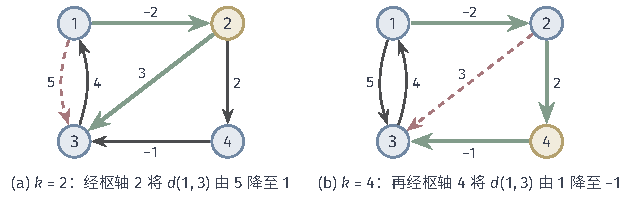
\includegraphics[width=107.184mm]{figures/03-graphs/02-combinatorial-optimization/tikz/floyd-warshall-example/figure.pdf}
  \caption{四顶点含负边有向图上Floyd--Warshall算法的逐层更新示例。黄色节点为当前阶段新开放的中间枢轴顶点$k$，绿色粗弧为当前阶段得到的$1\to 3$最短路线，红色虚弧为被替代的旧路线。(a) 阶段$k=2$开放顶点$2$后，绕行$1\to 2\to 3$（权和$-2+3=1$）替代直达弧$1\to 3$（权$5$）。(b) 阶段$k=4$开放顶点$4$后，绕行$1\to 2\to 4\to 3$（权和$-2+2-1=-1$）进一步替代$1\to 2\to 3$。}
  \label{fig:floyd-warshall-example}
\end{BookInlineFigure}

\subsubsection{算法分析}

\paragraph{正确性证明与就地更新次序}
我们先用对阶段$k$的数学归纳法证明递推式~\eqref{eq:floyd-warshall-recurrence}的正确性，再说明为何单数组就地更新不会破坏归纳假设。

\begin{theorem}[Floyd--Warshall算法的正确性]
\label{thm:floyd-warshall-correctness}
设有限有向加权图$\mathcal G=(V,E,w)$不含负环。对每个$k\in\{0,1,\ldots,n\}$及任意$i,j\in V$，由式~\eqref{eq:floyd-warshall-recurrence}递推得到的$d^{(k)}(i,j)$恰好等于从$i$到$j$且中间顶点均属于$\{1,\ldots,k\}$的最短路长度；特别地，算法~\ref{alg:floyd-warshall}结束时的$d(i,j)=d^{(n)}(i,j)=d^*(i,j)$。若图中存在负环，算法结束时必存在某个顶点$i$满足$d(i,i)<0$。
\end{theorem}

\begin{proof}
先设图中不含负环，对$k$进行归纳。当$k=0$时，中间顶点集$\{1,\ldots,k\}$为空集，从$i$到$j$不经过任何中间顶点的路径只有零步路径（$i=j$，成本$0$）或单条直达弧$i\to j$（成本$w(i,j)$），这与初始值$d^{(0)}(i,j)$的定义完全一致。

假设结论对$k-1$（$k\geq1$）成立。记$\mathcal P^{(k)}_{i,j}$为从$i$到$j$且中间顶点均属于$\{1,\ldots,k\}$的简单路径集合。由于不含负环，该限制下的最短行走可消去所有非负闭行走而化归为简单路径。一方面，$d^{(k-1)}(i,j)$对应一条中间顶点在$\{1,\ldots,k-1\}$内的路径，$d^{(k-1)}(i,k)+d^{(k-1)}(k,j)$对应将$i\leadsto k$与$k\leadsto j$两段中间顶点在$\{1,\ldots,k-1\}$内的路径在$k$处拼接所得的行走（其内部顶点属于$\{1,\ldots,k\}$），因此右端两项都是合法的候选成本，故$d^{(k)}(i,j)$不小于真实最优值。另一方面，任取一条达到该限制下最小成本的简单路径$P\in\mathcal P^{(k)}_{i,j}$：若$k$不是$P$的中间顶点，则$P\in\mathcal P^{(k-1)}_{i,j}$，由归纳假设其成本等于$d^{(k-1)}(i,j)$；若$k$是$P$的中间顶点，因$P$是简单路径，$k$在$P$内部仅出现一次，将$P$在$k$处切分为$P_1\in\mathcal P^{(k-1)}_{i,k}$与$P_2\in\mathcal P^{(k-1)}_{k,j}$，由归纳假设$w(P)=w(P_1)+w(P_2)\geq d^{(k-1)}(i,k)+d^{(k-1)}(k,j)$。综合两方面，式~\eqref{eq:floyd-warshall-recurrence}在阶段$k$精确成立。取$k=n$即得$d^{(n)}(i,j)=d^*(i,j)$。

再说明为何算法~\ref{alg:floyd-warshall}省略上标$(k)$、在单个二维数组$d(i,j)$上就地更新时结果完全不变。在第$k$轮内层循环中，更新$d(i,j)$读取的是同一轮中的$d(i,k)$和$d(k,j)$。注意当$j=k$时，候选值为$d^{(k-1)}(i,k)+d^{(k-1)}(k,k)$；在无负环假设下$d^{(k-1)}(k,k)=0$，故$d^{(k)}(i,k)=\min\{d^{(k-1)}(i,k),\,d^{(k-1)}(i,k)+0\}=d^{(k-1)}(i,k)$，同理$d^{(k)}(k,j)=d^{(k-1)}(k,j)$。也就是说，在第$k$轮迭代中，第$k$列元素$d(\cdot,k)$与第$k$行元素$d(k,\cdot)$的值根本不会改变。因此在更新任意位置$(i,j)$时，无论$(i,k)$或$(k,j)$在本轮中是先于$(i,j)$扫描还是后于$(i,j)$扫描，读取到的$d(i,k)$和$d(k,j)$都恒等于上一轮结束时的$d^{(k-1)}(i,k)$和$d^{(k-1)}(k,j)$，不会发生同轮覆盖污染。

最后，即使存在负环，按最大内部顶点拆分一条简单路径并归纳，仍可证明：当其内部顶点均已开放时，距离标签不大于这条路径的成本；就地更新只会进一步降低标签。若图中存在简单负环$C$，取$C$上编号最大的顶点记为$k^*$，取$C$上另一顶点$i^*$。$C$从$i^*$经$k^*$回到$i^*$，除$k^*$外其余顶点编号均小于$k^*$，故在阶段$k^*-1$结束时已有$d^{(k^*-1)}(i^*,k^*)+d^{(k^*-1)}(k^*,i^*)\leq w(C)<0$，从而在第$k^*$轮更新后$d(i^*,i^*)<0$；此后标签只降不升，算法结束时必检测到$d(i^*,i^*)<0$。
\end{proof}

上述关于就地更新的分析同时解释了一个常见的实现陷阱：\emph{三重循环的嵌套次序必须是$k$在最外层、$i$与$j$在内层（$k\to i\to j$），绝不能把循环次序调换为$i\to j\to k$}。若将$i,j$放在外层而只在最内层遍历$k=1,\ldots,n$，那么当固定一对$(i,j)$尝试用$d(i,k)+d(k,j)$更新$d(i,j)$时，其它顶点对$(i,k)$或$(k,j)$若排在$(i,j)$之后，就还未经过中间顶点$1,\ldots,k-1$的松弛更新，从而漏掉了大量需要多跳中转的最短路径。例如在前面的四顶点算例中，最短路径$2\to 4\to 3\to 1$依次经过编号为$4$和$3$的中间顶点（编号递减）；若外层先固定$(i,j)=(2,1)$再令$k=1,2,3,4$单趟递增，当检查$k=3$时$d(2,3)$尚未借$k=4$从$3$降为$1$，而当检查$k=4$时$d(4,1)$在初始表中还是$+\infty$，最终算出的$d(2,1)$将停留在错误的$7$而非真实的$5$。只有把$k$放在最外层，才能保证在进入阶段$k$之前，\emph{所有}顶点对的$d^{(k-1)}(\cdot,\cdot)$都已经完整算出。

\paragraph{时间与空间复杂度}
算法~\ref{alg:floyd-warshall}有三层至多运行$n$次的循环，最内层执行常数次运算，故最坏时间复杂度为$\Theta(n^3)$。本算法会跳过不可达的$i,k$组合，特定稀疏实例的实际工作量可能更少。距离矩阵与前驱矩阵各占$\Theta(n^2)$空间。规则的矩阵访问便于实现，但具体运行速度仍取决于数据布局、硬件与实现方式。

\subsection{Johnson算法}
\label{sec:johnson-algorithm}

\subsubsection{问题与思路}

当图是边数$m\ll n^2$的稀疏图（如道路网或大规模稀疏网络，$m=O(n)$）且含有负权弧时，Floyd--Warshall算法的$\Theta(n^3)$最坏时间上界可能高于利用稀疏性的算法。我们在第~\ref{sec:apsp-problem}小节看到，若能对每个源点运行一次Dijkstra算法，$n$次查询仅需$O(nm+n^2\log n)$时间；需要处理的障碍是图中的负权弧。于是自然产生这样一个问题：能否对图上每条弧的权值$w(u,v)$做一次变换，生成一组全新的\emph{非负}弧权$\tilde w(u,v)\geq0$，并且保证新权值下的最短路径与原权值下的最短路径完全相同？

初学者最容易想到的一种朴素方案是“全局平移”：找出全图最负的边权$-C$（其中$C>0$），把每一条弧的权值统一加上常数$C$，令$w'(u,v)=w(u,v)+C\geq0$。遗憾的是，这种平移会\emph{改变最短路径本身}。原因在于，一条包含$k$条弧的路径$P$，在新权值下的总长度会变成$w'(P)=w(P)+kC$：经过的弧数$k$越多，被额外追加的惩罚$kC$就越大。例如从$s$到$t$有一条直达弧（权$2$，含$1$条弧）和一条经过两个中转点的三弧路线（各段权$2,2,-3$，总权$1$，含$3$条弧），原本三弧路线更短（$1<2$）；若为消去$-3$而给每条弧统一加上$C=3$，直达弧新权变为$2+3=5$，而三弧路线被加上了$3\times3=9$，新总权变成$1+9=10>5$，原本的最短路反而被误判为更长。

朴素平移之所以失败，是因为路径的附加量$kC$取决于路径的内部边数$k$。要想让连接同一对起点$s$和终点$t$的所有路径在变换后增加完全相同的常数（与路径内部经过多少条弧、走哪条路线无关），每条弧的改变量就必须在路径拼接时“首尾相消”。这正是引入\term{顶点势}（vertex potential，亦称势函数）的核心动机：为每个顶点$v\in V$赋予一个实数势$h(v)\in\mathbb R$，并将每条弧$(u,v)\in E$的\term{约化权}（reduced weight，在流网络中对应第~\ref{chap:min-cost-flow}章的约化费用）定义为
\begin{equation}
  \tilde w(u,v) = w(u,v) + h(u) - h(v).
  \label{eq:johnson-reduced-weight}
\end{equation}

考察任意一条从起点$s=v_0$到终点$t=v_k$的路径$P=(v_0,v_1,\ldots,v_k)$。将路径上各段弧的约化权相加，所有内部顶点$v_1,\ldots,v_{k-1}$的势函数一负一正恰好裂项相消（telescoping sum）：
\begin{equation}
  \begin{aligned}
    \tilde w(P) &= \sum_{r=1}^{k}\tilde w(v_{r-1},v_r)
    = \sum_{r=1}^{k}\bigl(w(v_{r-1},v_r) + h(v_{r-1}) - h(v_r)\bigr) \\
    &= \sum_{r=1}^{k}w(v_{r-1},v_r) + h(v_0) - h(v_k)
    = w(P) + h(s) - h(t).
  \end{aligned}
  \label{eq:johnson-telescoping}
\end{equation}
式~\eqref{eq:johnson-telescoping}表明：当固定起点$s$和终点$t$时，不管路径$P$中途绕了多少条边，它的新成本$\tilde w(P)$与原成本$w(P)$永远只相差一个仅依赖于端点$s,t$的固定常数$h(s)-h(t)$。因此，对于任意两组$s$--$t$路径$P_1,P_2$，有$\tilde w(P_1)\leq\tilde w(P_2)$当且仅当$w(P_1)\leq w(P_2)$；新权值$\tilde w$保持了所有顶点对之间的最短路径集合。更进一步，对任意闭行走（或有向环）$C$，因其起点与终点相同（$s=t$），首尾势差$h(s)-h(s)=0$也一并抵消，得到$\tilde w(C)=w(C)$，即势函数重赋权保持每个有向环的总权值不变。

现在只剩下最后一个关键问题：怎样挑选这组顶点势$h:V\to\mathbb R$，才能使全图每一条弧$(u,v)\in E$的约化权都满足非负条件$\tilde w(u,v)\geq0$？将式~\eqref{eq:johnson-reduced-weight}改写为不等式，我们需要对每条弧$(u,v)\in E$同时满足
\begin{equation}
  h(v) \leq h(u) + w(u,v).
  \label{eq:johnson-triangle-ineq}
\end{equation}
对照第~\ref{sec:graph-opt-sp-relaxation}小节的最短路最优性证书式~\eqref{eq:graph-opt-shortest-path-certificate}，式~\eqref{eq:johnson-triangle-ineq}正是单源最短路距离天然满足的三角不等式。只要原图$\mathcal G$不含负环，我们只需在原图外添置一个虚拟\emph{超级源点}$s_0\notin V$，并从$s_0$向原图每个顶点$v\in V$各连一条权值为$0$的有向弧$s_0\to v$（构成扩展图$\mathcal G'=(V\cup\{s_0\},E\cup\{(s_0,v):v\in V\})$）。由于$s_0$没有任何入弧，新增的弧不会创造出任何新的有向环，$\mathcal G'$与$\mathcal G$具有完全相同的有向环，且原图每个顶点$v$都从$s_0$一步可达（距离至多为$0$）。在扩展图$\mathcal G'$上以$s_0$为源点运行一次Bellman--Ford算法：若算法报告存在可达负环，则原图$\mathcal G$必含负环；否则，取每个顶点的势为从$s_0$出发的最短路距离
\begin{equation}
  h(v) = d^*_{\mathcal G'}(s_0,v)\in\mathbb R,\qquad\forall v\in V,
  \label{eq:johnson-potential-choice}
\end{equation}
由最短路距离的三角不等式立即保证对一切$(u,v)\in E$都有$h(v)\leq h(u)+w(u,v)$，从而$\tilde w(u,v)=w(u,v)+h(u)-h(v)\geq0$恒成立。这就是1977年由Donald B. Johnson提出的\term{Johnson算法}（Johnson's algorithm）。

\subsubsection{算法实现}

Johnson算法的完整流程分为三个阶段：第一阶段构造超级源点$s_0$并调用一次Bellman--Ford算法，同时完成负环检测与顶点势$h(v)$的计算；第二阶段遍历全部有向弧计算非负约化权$\tilde w(u,v)$；第三阶段在非负权图$(\mathcal G,\tilde w)$上依次以每个顶点$u\in V$为源点调用Dijkstra算法求出重赋权后的最短距离$\tilde d^*(u,v)$，最后利用逆变换$d^*(u,v)=\tilde d^*(u,v)-h(u)+h(v)$还原出原始权值下的真实全源最短距离矩阵。

\begin{algorithm}[Johnson全源最短路算法]
\label{alg:johnson-apsp}
输入：有向加权图$\mathcal G=(V,E,w)$。输出：全源最短距离矩阵$\bm D=(d^*(u,v))_{u,v\in V}$与前驱矩阵$\bm\Pi$，或报告“存在负环”。
\begin{enumerate}
  \item 构造扩展图与计算势函数：令$V'=V\cup\{s_0\}$，$E'=E\cup\{(s_0,v):v\in V\}$，对每个$v\in V$置$w(s_0,v)=0$。在$\mathcal G'=(V',E',w)$上以$s_0$为源点运行Bellman--Ford算法（算法~\ref{alg:graph-opt-bellman-ford}）。若检测到负环，报告“图中存在负环”并停止；否则对每个$v\in V$令$h(v)=d^*_{\mathcal G'}(s_0,v)$。
  \item 边权重赋权：对每条原图有向弧$(u,v)\in E$，计算非负约化权
  \[
    \tilde w(u,v) \gets w(u,v) + h(u) - h(v).
  \]
  \item 重复运行Dijkstra并还原距离：对每个源点$u\in V$：
    \begin{enumerate}
      \item 在非负加权图$(V,E,\tilde w)$上以$u$为源点运行Dijkstra算法（算法~\ref{alg:graph-opt-dijkstra}），得到距离向量$\tilde d^*(u,v)$与前驱$\pi(u,v)$（$\forall v\in V$）；
      \item 对每个终点$v\in V$，若$\tilde d^*(u,v)=+\infty$则置$d^*(u,v)=+\infty$，否则还原真实最短距离：
      \[
        d^*(u,v) \gets \tilde d^*(u,v) - h(u) + h(v).
      \]
    \end{enumerate}
  \item 返回距离矩阵$\bm D=(d^*(u,v))$与前驱矩阵$\bm\Pi=(\pi(u,v))$。
\end{enumerate}
\end{algorithm}

\paragraph{四顶点有向图算例的重赋权演示}
我们在与第~\ref{sec:floyd-warshall}小节完全相同的四顶点六弧有向图上演示算法~\ref{alg:johnson-apsp}（图~\ref{fig:johnson-reweighting}）。

第一步，引入超级源点$s_0$并连接四条零权弧$s_0\to 1,2,3,4$（图~\ref{fig:johnson-reweighting}a）。从$s_0$出发运行Bellman--Ford算法：到顶点$1$和$4$的最短路即零权直达弧，故$h(1)=0$、$h(4)=0$；到顶点$2$经由$s_0\to 1\to 2$取得最小成本$0+(-2)=-2$，故$h(2)=-2$；到顶点$3$经由$s_0\to 4\to 3$（或$s_0\to 1\to 2\to 4\to 3$）取得最小成本$0+(-1)=-1$，故$h(3)=-1$。所得顶点势向量为
\[
  \bigl(h(1),\,h(2),\,h(3),\,h(4)\bigr) = (0,\,-2,\,-1,\,0).
\]

第二步，按式~\eqref{eq:johnson-reduced-weight}逐条计算六条弧的约化权$\tilde w(u,v)=w(u,v)+h(u)-h(v)$（图~\ref{fig:johnson-reweighting}b）：
\[
  \begin{aligned}
    \tilde w(1,2) &= -2 + 0 - (-2) = 0, &\qquad \tilde w(1,3) &= 5 + 0 - (-1) = 6, \\
    \tilde w(2,3) &= 3 + (-2) - (-1) = 2, &\qquad \tilde w(2,4) &= 2 + (-2) - 0 = 0, \\
    \tilde w(3,1) &= 4 + (-1) - 0 = 3, &\qquad \tilde w(4,3) &= -1 + 0 - (-1) = 0.
  \end{aligned}
\]
可以看到，原本为负的弧$1\to 2$（权$-2$）和$4\to 3$（权$-1$），连同位于从$s_0$出发的最短路树上的弧$2\to 4$，在重赋权后约化权全部变为$0$（对应势不等式取等），其余三条弧的约化权分别为$6,2,3$，全图所有弧权均已非负。

第三步，在非负权图$(V,E,\tilde w)$上从每个顶点$u\in\{1,2,3,4\}$分别运行Dijkstra算法：
\begin{itemize}
  \item 以$u=1$为源点：沿零权路径$1\to 2\to 4\to 3$，Dijkstra算法算出到全部四个顶点的约化最短距离均为$\tilde d^*(1,\cdot)=(0,0,0,0)$。代入还原公式$d^*(1,v)=\tilde d^*(1,v)-h(1)+h(v)=0-0+h(v)$，立即恢复出第$1$行真实距离$(0,-2,-1,0)$。
  \item 以$u=2$为源点：沿$2\to 4\to 3$得$\tilde d^*(2,4)=\tilde d^*(2,3)=0$，再经$3\to 1$（约化权$3$）得$\tilde d^*(2,1)=3$，即$\tilde d^*(2,\cdot)=(3,0,0,0)$。减去$h(2)=-2$并加上各终点势$h(v)$，还原得第$2$行真实距离$(3+2+0,\,0+2-2,\,0+2-1,\,0+2+0)=(5,0,1,2)$。
  \item 以$u=3$和$u=4$为源点：同理分别由Dijkstra算出$\tilde d^*(3,\cdot)=(3,3,0,3)$与$\tilde d^*(4,\cdot)=(3,3,0,0)$，还原后得到第$3$行$(4,2,0,4)$与第$4$行$(3,1,-1,0)$。
\end{itemize}
本例四次Dijkstra还原出的距离矩阵与前小节的$\bm D^{(4)}$一致，前驱矩阵也可取为所列的$\bm\Pi^{(4)}$。一般存在多条等长最短路时，不同算法的前驱矩阵可以不同。

\begin{BookInlineFigure}
  \centering
  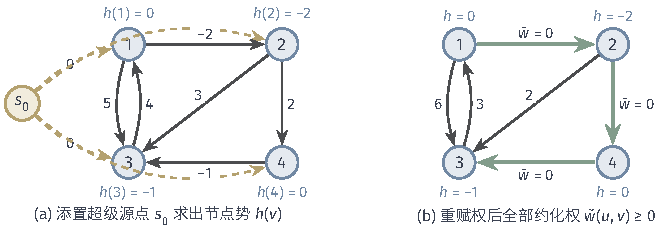
\includegraphics[width=112.843mm]{figures/03-graphs/02-combinatorial-optimization/tikz/johnson-reweighting/figure.pdf}
  \caption{Johnson算法在四顶点含负边有向图上的势函数重赋权过程。(a) 添置超级源点$s_0$（黄色）并向各点连零权虚线弧，运行一次Bellman--Ford得到顶点势$(h(1),h(2),h(3),h(4))=(0,-2,-1,0)$。(b) 按$\tilde w(u,v)=w(u,v)+h(u)-h(v)$重赋权后，原最短路树上的弧（绿色粗弧）约化权变为$0$，其余弧约化权为正数$6,2,3$，全图不含负权弧。}
  \label{fig:johnson-reweighting}
\end{BookInlineFigure}

\subsubsection{算法分析}

\paragraph{正确性与最优路径保持定理}
我们将前面的推导总结为如下定理。

\begin{theorem}[Johnson重赋权的非负性与最优路径保持]
\label{thm:johnson-correctness}
设有限有向加权图$\mathcal G=(V,E,w)$。
\begin{enumerate}
  \item 对任意给定的势函数$h:V\to\mathbb R$，由$\tilde w(u,v)=w(u,v)+h(u)-h(v)$定义的约化权保持所有顶点对之间的最短路径不变：一条$s$--$t$路径$P$在原权$w$下是最短路，当且仅当$P$在约化权$\tilde w$下是最短路；且有向环$C$满足$\tilde w(C)=w(C)$。
  \item 原图$\mathcal G$不含负环当且仅当扩展图$\mathcal G'$从超级源点$s_0$出发不含可达负环。此时取$h(v)=d^*_{\mathcal G'}(s_0,v)$均有限，且对每条弧$(u,v)\in E$均有$\tilde w(u,v)\geq0$，算法~\ref{alg:johnson-apsp}正确输出全源最短距离矩阵$\bm D$与前驱矩阵$\bm\Pi$。
\end{enumerate}
\end{theorem}

\begin{proof}
第1条由裂项恒等式~\eqref{eq:johnson-telescoping}直接给出：对固定端点$s,t$，任意$s$--$t$行走$W$满足$\tilde w(W)=w(W)+h(s)-h(t)$，两边对$W\in\mathcal W_{s,t}$取下确界即得$\tilde d^*(s,t)=d^*(s,t)+h(s)-h(t)$，且取到下确界的路径完全一致。闭行走满足$s=t$，故$\tilde w(C)=w(C)$。

下证第2条。因为$s_0$在$\mathcal G'$中入度为$0$，$\mathcal G'$中的任何有向环都不可能包含$s_0$，故$\mathcal G'$的有向环集合与$\mathcal G$完全相同；又因$s_0$有直达弧通向$V$中每个顶点，$\mathcal G$中任何负环在$\mathcal G'$中都从$s_0$可达。当无负环时，由于存在零权弧$s_0\to v$，有$-\infty<d^*_{\mathcal G'}(s_0,v)\leq0$，故$h(v)$必为有限实数。对任意$(u,v)\in E$，从$s_0$到$u$的最短路接上弧$u\to v$构成一条从$s_0$到$v$、成本为$h(u)+w(u,v)$的行走，由最短距离的下界性质得$h(v)\leq h(u)+w(u,v)$，移项即$\tilde w(u,v)=w(u,v)+h(u)-h(v)\geq0$。既然$\tilde w\geq0$，第三步中每次调用Dijkstra算法都能正确求出$\tilde d^*(u,v)$（定理~\ref{thm:graph-opt-dijkstra}），再经$d^*(u,v)=\tilde d^*(u,v)-h(u)+h(v)$还原即得原图的精确距离。
\end{proof}

\paragraph{复杂度分析与后续章节的联系}
我们来核算算法~\ref{alg:johnson-apsp}的三步开销：第一步在含$n+1$个顶点、$m+n$条弧的扩展图$\mathcal G'$上运行一次Bellman--Ford算法，耗时$O(n(n+m))=O(nm+n^2)$；第二步重赋权遍历全部$m$条弧，耗时$O(m)$；第三步运行$n$次Dijkstra算法，若采用Fibonacci堆实现，单次耗时$O(m+n\log n)$，$n$次共耗时$O(nm+n^2\log n)$（若采用普通二叉堆实现，则为$O(n(n+m)\log n)$），最后还原$n^2$个距离值耗时$O(n^2)$。因此，Johnson算法的总时间复杂度为
\begin{equation}
  T_{\mathrm{Johnson}}(n,m) = O(nm + n^2\log n)\quad\text{（二叉堆实现下为 }O(n(n+m)\log n)\text{）},
  \label{eq:johnson-complexity}
\end{equation}
除存储输出的$n\times n$矩阵外，工作空间仅为$O(n+m)$。在$m=O(n)$的稀疏图上，Johnson算法耗时$O(n^2\log n)$，比Floyd--Warshall算法的$\Theta(n^3)$具有更低的渐近时间上界。

值得特别指出的是，Johnson算法中“利用顶点势调整边权、依靠路径裂项相消保持目标差值不变”的思想，并非全源最短路独有的技巧，而是贯穿本部分后续章节的一条核心主线。在第~\ref{chap:bipartite-matching-assignment}章的带权指派问题中，可行标号与物品价格正是二部图上的顶点势；到了第~\ref{chap:min-cost-flow}章（最小费用流），式~\eqref{eq:johnson-reduced-weight}中的约化权在取$\pi=-h$的记号约定后，对应残量网络上的“约化费用”$\bar c_{i,j}=c_{i,j}-\pi_i+\pi_j$（式~\eqref{eq:graph-opt-reduced-cost}），而逐次最短路算法每轮借节点势把残量弧费用维持为非负、从而反复调用Dijkstra算法增广的做法，更是Johnson势函数重赋权在流网络上的直接延伸。

\subsection{方法比较与结果检验}
\label{sec:apsp-comparison}

求解全源最短路的四种主要方案——$n$次Bellman--Ford、$n$次Dijkstra、Floyd--Warshall算法与Johnson算法——在适用条件、数据结构依赖和渐近复杂度上各有侧重，表~\ref{tab:apsp-methods-comparison}将它们并列对比。

\begin{table}[!htb]
  \centering
  \begin{tabular}{@{}lllll@{}}
    \toprule
    方法 & 允许负权弧 & 负环检测 & 时间复杂度 & 典型适用场景 \\
    \midrule
    $n$次Dijkstra & 否（要求$w\geq0$） & 不适用 & $O(nm+n^2\log n)^*$ & 非负权稀疏图 \\
    $n$次Bellman--Ford & 是 & 支持 & $O(n^2+n^2m)$ & 仅作基准对照 \\
    Floyd--Warshall & 是 & 对角线$d(i,i)<0$ & $\Theta(n^3)$ & 稠密图、矩阵/小规模图 \\
    Johnson算法 & 是 & 超级源点BF检测 & $O(nm+n^2\log n)^*$ & 含负权弧的稀疏图 \\
    \bottomrule
  \end{tabular}
  \caption{全源最短路求解方法的比较（$n=|V|$为顶点数，$m=|E|$为有向弧数；带$^*$号为Fibonacci堆界，使用二叉堆时为$O(n(n+m)\log n)$，稠密图用数组扫描版Dijkstra为$O(n^3)$）。}
  \label{tab:apsp-methods-comparison}
\end{table}

选择算法时，先检查弧权条件和输出需求。非负权图可以逐源运行Dijkstra算法；含负权弧时，Floyd--Warshall与Johnson都可检测负环，在无负环时返回全源距离。稠密图上可比较Floyd--Warshall与数组版Dijkstra的立方时间实现，稀疏图上则可考虑Johnson。理论复杂度不能直接确定某个顶点数阈值下哪一种实现更快，具体选择还需结合存储与运行测量。

拿到一份无负环图上的全源最短路输出$(\bm D,\bm\Pi)$后，怎样不重跑算法而独立核对它的正确性？与第~\ref{sec:graph-opt-sssp-comparison}小节的单源检验一脉相承，核验分为“上界可达到”与“下界最优性”两步：
\begin{enumerate}
  \item 可达性见证（$d(u,v)\geq d^*(u,v)$）：对每个源点$u\in V$，检查$d(u,u)=0$，并对每个满足$d(u,v)<+\infty$且$v\neq u$的顶点$v$，验证前驱边$(\pi(u,v),v)\in E$、前驱链不形成有向环且满足等式
  \[
    d(u,v) = d\bigl(u,\pi(u,v)\bigr) + w\bigl(\pi(u,v),v\bigr).
  \]
  这保证沿着$\bm\Pi$的第$u$行回溯必能到达$u$，且该路径的真实弧长之和恰好等于$d(u,v)$。
  \item 逐弧三角不等式证书（$d(u,v)\leq d^*(u,v)$）：对每个源点$u\in V$与图中的每条有向弧$(x,y)\in E$，核对三角不等式
  \begin{equation}
    d(u,y) \leq d(u,x) + w(x,y).
    \label{eq:apsp-certificate}
  \end{equation}
  只要式~\eqref{eq:apsp-certificate}对所有$u\in V$和$(x,y)\in E$成立，沿任意$u\leadsto v$路径累加即证$d(u,v)\leq d^*(u,v)$。两步合在一起，仅需$O(n(n+m))$时间即可完成对全源最短路矩阵$(\bm D,\bm\Pi)$的完备检验。
\end{enumerate}

% 第3章：本章小结。
\FloatBarrier
\section{本章小结}
\label{sec:graph-opt-sp-summary}
\label{sec:shortest-paths-summary}
\label{sec:apsp-summary}

本章围绕有向加权图上的最短路问题，先后解决了从单一源点出发的单源最短路问题，以及同时求所有顶点对距离的全源最短路问题。

在共同基础（第~\ref{sec:shortest-path-foundations}节）中，按有限行走成本的下确界定义最短路距离后，每个有序顶点对$(s,v)$的距离属于三类之一：不可达时为$+\infty$；可达且不受负环影响时为有限值，并由一条简单路径达到；能从某个$s$可达的负环到达时为$-\infty$。负环只影响能从源点经该环到达的终点。各类算法共用的核心机制是距离标签与逐弧松弛：标签从“源为零、其余为无穷”出发，只通过松弛下降，因而始终是有实际路线见证的距离上界；而当所有弧都满足三角不等式$d(v)\leq d(u)+\ell_{u,v}$时，沿任意行走裂项相加又给出距离下界，两者合一即构成不依赖算法过程的最优性证书。

在单源最短路（第~\ref{sec:single-source-shortest-paths}节）中，三种算法的差别在于何时能认定标签不再改变，而这取决于输入图的环结构与边长符号。有向无环图按拓扑序处理，前驱的距离在使用前已经确定，弧长可取任意实数，总时间$O(n+a)$，编辑距离一类的状态递推正是这种情形。

Bellman--Ford算法不要求无环，同步版本第$k$轮的标签恰是至多$k$条弧的最优值，$n-1$轮后仍能改善的弧暴露负环的影响，就地更新版本总时间$O(n+na)$，直接复制数组的同步版本为$O(n(n+a))$。

Dijkstra算法要求可达部分弧长非负，每次出队的最小标签顶点立即永久确定，用二叉堆时为$O((n+a)\log n)$；哪怕没有负环，一条负边就可能使它过早锁定标签而出错。

在全源最短路（第~\ref{sec:all-pairs-shortest-paths}节）中，为了突破含负边图上重复运行$n$次Bellman--Ford算法的$O(n^2+n^2m)$时间上界，本章建立了两条互补路线。

其一是面向稠密图与矩阵计算的Floyd--Warshall算法：它按允许经过的中间顶点编号集合$\{1,\ldots,k\}$逐层递推，利用简单路径至多经过枢轴顶点$k$一次的性质做二选一更新，在代数上对应$(\min,+)$热带半环上的矩阵消元；就地更新须把$k$放在最外层，$i,j$两层可以互换，由对角线$d(i,i)<0$检测负环，最坏时间为$\Theta(n^3)$、空间为$\Theta(n^2)$。

其二是面向含负边稀疏图的Johnson算法：它引入顶点势$h(v)$定义约化权$\tilde w(u,v)=w(u,v)+h(u)-h(v)$，依靠路径裂项相消保持最短路与环权不变；通过添加超级源点$s_0$运行一次Bellman--Ford取$h(v)=d^*_{\mathcal G'}(s_0,v)$，由三角不等式保证$\tilde w(u,v)\geq0$，随后调用$n$次Dijkstra算法将总时间降至$O(nm+n^2\log n)$。

下一章（第~\ref{chap:minimum-spanning-tree}章）转向另一种选择对象：最小生成树比较的是一整组连通边的总造价，而不是两点间路线的长度。本章建立的逐弧三角不等式与Johnson势函数重赋权，则会在第~\ref{chap:bipartite-matching-assignment}章的可行标号和第~\ref{chap:min-cost-flow}章的节点势与约化费用中再次发挥核心作用。

